
\section{Introduction}
\vspace*{-5pt}

Compact binary coalescence is the most promising source of gravitational-waves
for Advanced LIGO~\cite{Abadie:2010cf}.  The inspiral and merger of a binary
containing stellar-mass compact objects (neutron stars and black holes)
generates gravitational waves that sweep upward in frequency and amplitude
through the sensitive band of Advanced LIGO. Compact binary coalescence
searches in Initial
LIGO~\cite{LIGOS1iul,Abbott:2005pe,Abbott:2005kq,Abbott:2005qm,Abbott:2007ai,Abbott:2009tt,Abbott:2009qj,Abadie:2010yb,Collaboration:S5HighMass,Colaboration:2011np,Aasi:2013jjl}
were performed by a high-latency (or deep, offline) search pipeline. For Advanced LIGO, both high-latency offline deep searches and low-latency rapid-result searches will be performed. The
offline search pipeline performs: (i) initial analysis of LIGO data with and
without simulated signals to measure detector performance and tune the
parameters for a deep search; (ii) full analysis of the data set with the
final search parameters to detect signals and measure the false alarm rate of
detection candidates; and (iii) reanalyzing the data with the addition of a
large number of simulated signals to determine LIGO's sensitivity and
selection bias to the astrophysical population.
The high-latency CBC search incorporates information not available in the
low-latency search (for example, improved detector calibration information and
data quality information from offline detector characterization). It also
calculates detection probabilities using large,
time-symmetric samples of the detector noise background and performs a deep,
comprehensive search over the full parameter space of compact binaries.
%whereas the low-latency search pipeline only targets a the sources where an
%electromagnetic counterpart is expected.  
%The high-latency pipeline also
%ensures that any data lost to the low-latency pipeline through data dropouts
%or processing errors is included in the final search.  
The offline search 
measures the selection bias of the CBC search, including the loss in detection
efficiency caused by uncertainties in the model waveforms, or the omission of
certain physics (e.g. binary precession) in the detection templates.  In the
absence of a detection in a given region of the parameter space, the deep offline
search pipeline computes upper limits on the rate of CBC sources which can be
used to constrain astrophysical models of binary and compact object formation.
Consequently, both the deep, offline and the low-latency pipelines are
required to achieve Advanced LIGO's science goals. 

This document describes the computational cost of the high-latency CBC search,
which has been substantially re-written for Advanced LIGO. The prioritized request for computing 
for binary neutron star, neutron star--black hole,
and binary black hole sources is summarized in
Table~\ref{t:offline-xsede-request} (in Intel\textsuperscript{\textregistered} E5-2670 core
hours per year). For reference, we include the request from Table~3 of
LIGO-T1400269 presented in May 2014\footnote{The May 2014 offline CBC request
in LIGO-T1400269
was presented in Stampede SU, which assumes that a core is an Intel\textsuperscript{\textregistered} E5-2680.  For
direct comparison in Table~\ref{t:offline-xsede-request}, we convert this
request to E5-2670 cores by multiplying Stampede SU by the ratio of the clock
speeds, i.e. $2.7/2.6$.}.



\begin{table}[!t]
\centering
{\small
\begin{tabular}{|l|l|l|l|}
\hline 
{\bf Astrophysical search target}  & \multicolumn{3}{l|}{\bf E5-2670 MSU per year}\\

{ } &  {\bf 2015--16} & {\bf 2016--17} & {\bf 2017--18}  \\\hline\hline
{ Highest priority:\, Binary neutron stars (non-spinning templates)} & 0.084 & 0.514 & 1.48 \\\hline
{ High priority: Binary neutron stars (aligned-spin templates)} & 1.25 & 8.82 & 30.2 \\\hline
{ \it May 2014 Request: Binary neutron stars (aligned-spin templates)} & \it 44.4 & \it 130 & \it 270 \\\hline\hline
{ Highest priority: Neutron star--black hole (aligned spin templates) } & 2.26 & 17.5 & 65.7 \\\hline
{ \it May 2014 Request: Neutron star--black hole (aligned spin templates) } & \it 47.1 & \it 167 & \it 494 \\\hline\hline
{ Highest priority: Binary black hole search  (aligned spin templates) } & 1.45 & 11.9 & 36.1 \\\hline
{ \it May 2014 Request: Binary black hole search  (aligned spin templates) } & \it 23.5 & \it 72.3 & \it 151 \\\hline\hline
{ \bf Total for all high-latency CBC searches } & \bf 5.04 & \bf 38.7 & \bf 133 \\\hline
{ \it May 2014 Total for all high-latency CBC searches } & \it 115  & \it 369 & \it 915 \\\hline
\end{tabular}
}
\caption{\label{t:offline-xsede-request}
The computational resources needed to achieve the LVC's
production high-latency CBC search in millions of service units (MSU) per
year. One service unit is defined as one core hour on an Intel\textsuperscript{\textregistered} 
E5-2670. 
%Note the non-spinning binary neutron star search is a sub-set of the
%aligned spin binary neutron star search, so only one of these searches will be
%performed. 
Shown below each science goal (in italics) is the size of the
corresponding May 2014 request from Table 3 of LIGO-T1400269; the difference from May 2014 to April 2015 reflect optimization of code and the flow down of science priorities. Since no search
pipeline for precessing searches exists, this search is currently not listed
in the LSC's prioritized science goals.  Large-scale simulations included in
the above cost will allow us to measure the sensitivity of aligned-spin
searches to precessing systems.
}
\end{table}

We note that the computational resources requested here for the
high-latency CBC request are significantly less than those presented in the
May 2014 request, with the 2015/16 request being a factor of 23 smaller and
the 2017/18 request being a factor of 6.8 smaller. The majority of this
reduction is due to the significant improvements we have made in the new PyCBC
search executable, compared to the old LALApps search code. \textbf{The new
PyCBC code is a factor of $\mathbf{6.75}$ faster in terms of search throughput on our
reference CPU platform than search code used in Initial LIGO.} We describe the
optimizations that we have made to achieve this in detail in
Section~\ref{sec:CompAlgorithms}.

Further reductions are due to changes in the size of the template bank used in
the search, which changes computational cost linearly.  As a result of the scientific prioritization process and input
from the astrophysics community, we increased the minimum neutron star mass in
the binary neutron star and neutron star--black hole searches from $0.9\,
M_\odot$ to $1.0\, M_\odot$. This results in a template bank that is a factor of
$\sim 1.3$ smaller than that used in May 2014. Further reductions in the size
of the template bank are due to the use of a more refined noise curve than
that used in May 2014 to model the detector sensitivity.  
%Updated template
%banks computed using the more accurate noise curve models result in a factor
%of between $2.0$ and $1.1$ decrease in computational cost.  
Template banks computed using the more accurate noise model are a
factor of 1.1--2 times smaller.
We have also used a more realistic estimate of the detector observation time,
which reduces the requested computational resources by a factor of 2.4 in
2015--16, 1.8 in 2016--17, and 1.4 in 2017--18. We have also determined that a
larger number of simulated signals will be required to measure the efficiency
of the offline search than accounted for in the May 2014 request. This
increases our request by a factor of 1.6 in 2015--16, 2 in 2016--17, and 2.5
in 2017--18. However, the overall cost is still
substantially smaller than that presented last year.

There are several uncertainties in the computational cost
estimates presented here. The most significant uncertainty is the detector
sensitivity and bandwidth, as described in Section~\ref{sec:justification}. If
detector commissioning progresses at a more rapid pace and we achieve the best
expected Advanced LIGO sensitivity in O3, our computational cost would
increase by $\sim 50\%$. The throughput of the search code also depends on the
(as yet unknown) stationarity of the detector data, with more stationary data
having a faster throughput. If the data are very clean, then the
computational cost could be $\sim 20\%$ less than requested here. If the data
are very non-stationary, containing many non-Gaussian noise transients, then
the computational cost could increase by $\sim 40\%$. %(However, a reduction of
%this size is unlikely given on the quality of data seen to date from the
%Advanced LIGO detectors). 
We will continue to
refine our computational needs based on instrument progress and our best known
predictions for the detector's sensitivity evolution.

In addition to our optimization work on CPUs, we have also explored the use of
GPUs, which show significant promise for use in the high-latency CBC search.
The fastest throughput we have observed on a GPU with our initial CUDA kernels
is a factor of $\sim 3$ higher than the fastest throughput on a CPU socket. We
have also explored the use of consumer grade GPUs and have demonstrated that
these can yield an order of magnitude greater throughput per dollar than CPUs. Our
initial GPU kernels have not yet been fully optimized. We 
are collaborating with NVIDIA to increase their performance, as
described in Section.~\ref{sec:gpu-trade}.

Finally, we note that the scientific methods used for computational cost estimates
here are the same as those used for searches for gravitational waves
in Initial LIGO.  Reduction in computational costs described below therefore
result from optimization of the existing methods, prioritizing our science,
and better estimates of detector performance, rather than replacement of
Initial LIGO scientific methods with new ones. We have demonstrated that the
optimized code reproduces the results obtaining in Initial LIGO, but at
substantially reduced computational cost. This gives us confidence that the
optimized code described here will be successful in Advanced LIGO as we
explore new methods that may further reduce the cost and allow exploration of
larger parameter spaces (in particular, the space of precessing binaries).

The rest of this document is organized as follows:
Section~\ref{sec:methodology} reviews the high-latency CBC search pipeline and 
Section~\ref{sec:MethodSpace} describes the  scientific methods that
we have investigated to implement the high-latency CBC search.
Section~\ref{sec:CompMethod} describes the
data-analysis methods that dominate the computational cost of the search
pipeline (the matched filter and the time-frequency signal-based veto).
Section~\ref{sec:CompAlgorithms} discusses the selection of optimal
algorithms, libraries, and tests of our implementation on CPU hardware. In particular,
Section~\ref{sec:opt-chisq} describes an improved implementation of the
time-frequency signal consistency test, and Section~\ref{sec:opt-thresh}
describes an improved algorithm for event finding and clustering in the
matched filter output. Both of these improvements are independent of hardware
implementation. We then focus on optimization on the LIGO reference CPU, the
Intel\textsuperscript{\textregistered} E5-2670 (which is similar to the E5-2680 used in Stampede).
Section~\ref{sec:opt-fft} describes the selection of optimal FFT engines for
this hardware, and Sections~\ref{sec:parall-expens-kern} and
\ref{sec:vect-expens-kern} describe the improvements to parallelize and
vectorize the non-FFT portions of the filtering code. With these improvements,
we find that the fastest FFT method (eight core multi-threaded FFTW) provides
the greatest search throughput. Section~\ref{sec:perf-relat-theor} compares the
best measured performance with our theoretical expectations.
Based on the fastest CPU implementation on the E5-2670, and taking into account instrument and astrophysics tuning, Section~\ref{sec:justification} calculates the
resources required for the production high-latency CBC searches, as summarized
in Table~\ref{t:offline-xsede-request}.   Finally,
Section~\ref{sec:offline-trade-study} describes our hardware trade study
investigating performance on available CPU systems and, in
Section~\ref{sec:gpu-trade}, our implementation of the high-latency search on
Graphics Processing Units.

%~~~~~~~~~~~~~~~~~~~~~~~~~~~~~~
\vspace*{-10pt}
 \section{Compact Binary Coalescence Searches} 
\vspace*{-5pt}
 \label{sec:methodology}
%~~~~~~~~~~~~~~~~~~~~~~~~~~~~~~


If the angular momenta of the compact objects---their \emph{spins}---are
aligned with the orbital angular momentum of the binary (or the compact
objects are non-spinning), then the gravitational-wave strain $h$ observed by
LIGO or Virgo  (neglecting higher-order amplitude corrections) can be written as
\begin{equation}
h(t-t_c) = A(t - t_c) \cos( \phi(t - t_c) ) \cos \Phi - A(t - t_c) \sin( \phi(t - t_c) ) \sin \Phi,
\end{equation}
where $t_{c}$ is the coalescence time of the binary, $A \propto f_\mathrm{GW}^{2/3}$ is
the amplitude of the wave, $\Phi$ is a constant that depends on the
orientation of the binary, and $\phi$ is the time-evolving gravitational-wave
phase---the quantity to which LIGO and Virgo are most sensitive. The
gravitational-wave phase evolution is given by the particular waveform model
used in the search and depend only on the masses and spins of the compact
objects.  For detection of binaries with total mass $M \lesssim 12 M_\odot$ and spins $\chi
\lesssim 0.4$ (which includes binary neutron stars),  post-Newtonian theory
provides a sufficiently accurate analytic model of the gravitational
waveforms~\cite{Blanchet:2013haa,kidder:821,PhysRevD.47.R4183,Buonanno:2009zt,Brown:2012nn,Brown:2012qf}.
As the mass ratio and spins of the compact objects
increase~\cite{Brown:2012qf}, or the total mass of the binary
increases~\cite{Buonanno:2009zt,Brown:2012nn}, post-Newtonian waveforms 
become less accurate. In this case, we can model the signal
waveforms using analytic models methods, such as the effective one body (EOB)
approach~\cite{BuonannoDamour:1999} tuned to numerical relativity simulations of binary black holes~\cite{Taracchini:2013rva}, or by phenomenological models that capture the
dynamics of binary black holes~\cite{Hannam:2013oca,Purrer:2014fza}.

The amplitude of gravitational waves measured by the Advanced LIGO and Virgo detectors
is expected to be comparable to (or smaller than) the mean amplitude of the
detector noise.  Consequently, digital signal processing is required to
extract signals from the noisy detector data. For \ac{CBC} sources, it is
possible to construct models of the gravitational waveform. Matched
filtering~\cite{Wainstein:1962} would be the optimal method to identify
signals in the detector data, if the detector noise were stationary and
Gaussian. The noise in the LIGO and Virgo detectors from fundamental sources (thermal noise, radiation pressure noise, and photon shot noise) does behave in this way; however
populations of non-Gaussian, non-stationary transients of both environmental
and instrumental origin are also present. These ``glitches'' cause excursions in
the matched filter \ac{SNR} that may be mistaken for signals. Requiring that a
signal be seen in both LIGO detectors (and once running the Virgo detector) eliminates a substantial fraction of
false signals; however additional waveform consistency tests~\cite{Allen:2004gu}
are needed to determine if \ac{SNR} excursions are due to a glitch or a
gravitational wave~\cite{Babak:2012zx}. 
 

The gravitational waveform depends
sensitively on the mass and spin parameters of the source.  The parameters of
a signal are not known in advance, so 
a discrete ``bank'' of gravitational-waveform
templates~\cite{Owen:1998dk,Owen:1995tm,Balasubramanian:1995bm,Dhurandhar:1992mw,Sathyaprakash:1991mt} is constructed that is sensitive to the target astrophysical  population.
The computational cost of the search scales effectively linearly with the number
of templates in the bank, as the matched filter is applied once per template
in the bank. Template banks exist for binaries where the
angular momentum of the compact objects is negligible (non-spinning
binaries)~\cite{Cokelaer:2007kx,Babak:2006ty} and for the case in which the
component object's spin is aligned with the orbital angular momentum of the
binary~\cite{Brown:2012qf,Harry:2013tca}.
If the spin of the compact object is not aligned with the orbital angular
momentum (for example due to misalignment due to a supernova kick), spin-orbit
coupling will cause the plane of the binary to precess.  Spin-orbit and
spin-spin coupling also change the rate of energy and angular momentum loss
for the binary, which further changes the gravitational-wave signal.  
For binary neutron stars, a search for aligned-spin systems is sufficient to
capture precessing systems, as the effects of precession are not significant
for these systems~\cite{Brown:2012qf}.  However, for
binary black holes or neutron star--black hole binaries spin and precession
effects can be significant.  At present no template placement algorithm or
search pipeline has been implemented for spinning, precessing \ac{BBH} or \ac{NSBH}
binaries.  Search methods which incorporated spin effects were considered
in Initial LIGO, but were found to increase the false alarm rate 
resulting in a less sensitive
search~\cite{Pan:2003qt,Buonanno:2005pt,VanDenBroeck:2009gd}. Development of
precessing binary searches is an active topic of research, but these pipelines
are not yet in production for the LIGO-Virgo searches. In 
the absence of a search for precessing binaries, simulated signals from
a population of precessing binaries will allow us to quantify
the sensitivity of the LIGO-Virgo current search to the astrophysical population.

The full search for coalescing compact binaries requires: (i) generation of the
gravitational-wave template bank~\cite{Babak:2006ty,Brown:2012qf}; (ii) filtering
the data against this bank and identifying ``triggers'', or times where the
matched filter \ac{SNR} exceeds a certain threshold for a
particular template~\cite{Allen:2005fk}; (iii) checking triggers for consistency
using waveform consistency tests~\cite{Allen:2004gu}; (iv) folding in
information from instrumental health and status information to further
eliminate triggers due to instrumental
artifacts~\cite{Slutsky:2010ff,Aasi:2012wd-2}; (v) applying coincidence algorithms
to ensure that a gravitational-wave signal is present in two or more detectors
with consistent signal parameters; and (vi) measuring the significance of a
candidate signals by comparing their amplitude to that of the noise-induced
background.   Executing all of the above steps is the job of the \emph{analysis
pipeline}~\cite{Babak:2012zx,Brown:workflow}, a program that generates a
workflow that turns the raw detector data into a detection statement or
measures the signal parameters. The search pipeline is a heterogeneous mixture
of computational components that perform the required steps on all of the data
in the correct order. LIGO-specific scripts write workflows that are planned
by the Pegasus Workflow Management System into directed acyclic graphs (DAGs) that are executed by
HTCondor's DAGman. 
The computational cost of the full pipeline is dominated by the executable that
computes the matched filter and the waveform consistency tests. Based on a test
filtering 11.5 days of simulated Advanced LIGO data, we find that 99.8\% of the total 3727.63 core-days of runtime is spent in the \texttt{pycbc\_inspiral} filtering engine (that computes the templates, the correlation, the FFT, and event finding and clustering), with the remainder spent in the
coincidence, background estimation, and post-processing steps. Consequently,
we have focused our optimization efforts to date on the filtering executable
(although improvements have also been made to other parts of the pipeline).

A complication encountered when
benchmarking the offline CBC search is that the run time of the search  depends on the quality
of the (random) detector noise. To save computational cost, the filtering
executable only computes waveform consistency checks when the \ac{SNR} exceeds
a threshold value. However, we do not know in advance the character or the
rate of non-stationary noise transients in the data. Indeed, this rate can
change over time during an observing run.  To compute the computational cost
of the analysis, we take the average of the measured throughput over three
representative types of data. 

% Investigation of early
%Advanced LIGO data from the Livingston detector indicates that this is a
%reasonable assumption for the (as yet unknown) quality of data in the first
%Advanced LIGO observing run. 

% FIXME
%\todo{is it possible, and interesting, to put a number to the consequences for very good (Gaussian) noise performance or very poor (really glitchy) performance? is this by any chance a potential need for shared resources?}\todo{dhs more generally, need paragraphs here and there, and also in the Exec Summ, that acknowledge the uncertainty in the computing costs due to the instrument performance: both tuning choices, AND data quality. We want the NSF to be primed to hear that as a reason for potentially large changes in the total request.}

%To account for this, we benchmark the code
%on three types of data (labeled A, B, and C) from Initial LIGO, which are
%representative of different types of data quality: (i) a clean stretch of data
%(Type A); (ii) a stretch containing a single loud transient glitch (Type B);
%and (iii) a stretch with elevated levels of non-Gaussian noise at low
%frequencies (Type C).  Type C is the worst type of data quality in terms of
%computational cost. The speed of the analysis is significantly slower for this
%type of data, as more time is spent computing signal based vetoes. 



%~~~~~~~~~~~~~~~~~~~~~~~~~~~~~~
\section{Exploring the space of appropriate scientific methods}
\vspace*{-5pt}
\label{sec:MethodSpace}
%~~~~~~~~~~~~~~~~~~~~~~~~~~~~~~

The scientific methods used in the pipeline may be implemented by more than one computational
algorithm. For example, the matched filter signal-to noise ratio for a bank of
templates may be constructed by a frequency-domain correlation or linear
combinations of time domain correlations with an orthonormal filter set found
via the singular value decomposition (SVD).  Benchmarking of the LLOID
algorithm~\cite{Cannon:2011vi} (which uses SVD and muti-rate filtering to implement a low-latency
search as described in LIGO-T1400542) versus the frequency-domain FFT~\cite{Allen:2005fk}
has shown that the FFT method has a higher
template-per-core throughput for a given input data sample rate.   We have
therefore selected the frequency-domain FFT correlation as the optimal
scientific method to search for signals with the deep, offline pipeline where
latency is not a concern. Since the LLOID method is used to search for signals with a
possible rapid electromagnetic counterpart, it is appropriate to trade
computational cost for latency in the low-latency search.

Non-Gaussian noise transients in the detector data can cause the matched filter
to generate false triggers, and so a variety of \emph{signal-based vetoes}
have been developed that use additional information to distinguish signals
from noise. These are often called $\chi^2$-vetoes, as the three primary tests
considered (known as the time-frequency signal-based veto, the autocorrelation
signal-based veto, and the template bank veto) all generate a statistic that is
$\chi^2$ distributed in Gaussian noise. The low-latency CBC search implements
the autocorrelation signal-based veto, as it is straightforward to compute in
the low-latency search given its locality in time and dependence only on the
SNR time-series.
The offline search used in Initial LIGO
CBC searches (and used for cost estimates in the May 2014 review) computed the
time-frequency $\chi^2$ veto and the bank veto. The time-frequency $\chi^2$ veto
has been demonstrated to be a powerful test and is essential to eliminate
non-Gaussian transients from the search.  However, it has not been
demonstrated that the bank veto provides additional noise rejection power
beyond the time-frequency $\chi^2$ veto.  It has therefore been decided to
eliminate the computation of the bank veto from the filtering to save
computational cost.
We are also exploring the use of the autocorrelation $\chi^2$ veto (used in
the low-latency search) in the deep, offline search. Preliminary
investigations with prototype code suggest that this may provide additional information to the
time-frequency $\chi^2$ test for certain types of noise events, however it is
not yet clear if this veto provides more noise-rejection power than the standard
time-frequency $\chi^2$.

Two further refinements of the  scientific methods and tuning used in Initial
LIGO are being explored: (i)  In Initial LIGO, the search algorithm processed
fifteen data segments of length 256 seconds though each template, with noise
power spectral density (PSD) estimation performed over 2048 seconds. The new
\texttt{pycbc\_inspiral} executable allows us more control over the PSD
estimation, as well as the number and length of the filter data segments.
Preliminary investigations with increasing the length of the data segment to
512 seconds have shown a performance increase of $\sim 25\%$, as longer data
segments allow us to make more efficient use of the matched filter output by
decreasing the amount of time per data segment corrupted by the wrap-around
of the FFT; (ii) Re-using the template for more data segments also further
reduces the overall cost of the code. If Advanced LIGO provides sufficient
long, stable lock stretches, we can increase the number of data segments per
template, further reducing the overall search cost.

Moving beyond the existing methods, we are developing a new
matched-filtering algorithm that performs a search that is hierarchical in
sample rate.  An approximate signal-to-noise time series is first created by
reducing the sample rate, allowing the use of shorter, faster FFTs. Peaks of
interest are found using a threshold that has been lowered to account for both
the loss of the high frequency contribution to the SNR and the time offset
from the full sample rate peak.  Full sample rate matched filtering is
performed at these peaks and the nearby points, to minimize the probability
that the full sample rate peak is missed.  This step is accelerated using a
pruned FFT algorithm, where we decompose an N points FFT into a batched set of
FFTs  each $N^{(1/2)}$ in length, followed by an explicit DFT calculated for
every point. A further optimization removes the first memory transposition of
the FFT by storing the input data in a memory layout that is already
transposed for the first batched FFT. This algorithm is efficient due to the
small ratio between the number of interesting points to calculate and the number of points in
the full time series, $O(10^{-4})$, which allows us to make more efficient use
of the Level 3 cache.

This method performs an accurate approximation to the full matched filter;
however, it does not exactly reproduce the same output. Consequently, this
method require careful testing before it can be commissioned as a production
search. % to quantify any possible loss in event rate due to the hierarchical
%algorithm. 
A prototype implementation has been tested in the binary black
hole search, with the initial version of the code showing a 2--3 times speedup over the full
sample-rate computation of the matched filter. Ongoing work to develop this
method includes
increasing the efficiency of the full sample rate reconstruction which will
allow this algorithm to be efficient in the widest parameter space range. If
this new method can be demonstrated to yield the same detection efficiency as
the current methods, we will adopt it for Advanced LIGO, further reducing
computational cost.


%~~~~~~~~~~~~~~~~~~~~~~~~~~~~~~
\vspace*{-10pt}
\section{Computational Methods}
\vspace*{-5pt}
\label{sec:CompMethod}
%~~~~~~~~~~~~~~~~~~~~~~~~~~~~~~

The computational cost of the CBC search is dominated by the
\textsc{findchirp} matched filtering algorithm~\cite{Allen:2005fk} that
computes the matched-filter SNR and the waveform consistency test for a single
detector; combining these triggers from multiple detectors is relatively
inexpensive.
The matched-filter \ac{SNR} $\rho^2$ for the data $s$ and template $h$, analytically
maximized over $A$ and $\Phi$, is given by
%
\begin{equation}
\label{eq:cbc_snr}
\rho^2 = \frac{ (s|h_0)^2 + (s | h_{\pi/2})^2 }{(h_0|h_0)}; \quad
\textrm{with} \quad
(a|b) = 4 \, \mathrm{Re} \int_{f_{\mathrm{low}}}^{f_{\mathrm{high}}}
\frac{\tilde{a}(f) \, \tilde{b}^{*}(f)}{S_n(f)} df,
\end{equation}
%
where $S_n(f)$ the one-sided detector-noise \ac{PSD} and $h_0$ and $h_{\pi/2}$
correspond to the two gravitational-wave polarizations. 
If a gravitational wave signal is present in the data, then its location in time is
defined by the parameter $t_c$. To search over all possible
times $t_c$, we use a Fast Fourier Transform to compute the value of the inner product $(s|h_0)$ by
\begin{equation}
(s|h_0(t_c)) = 2 \int_{-\infty}^\infty\,df e^{2\pi ift_c}
\frac{\tilde{s}(f)\tilde{h}_0^\ast(f)}{S_n(|f|)}
\label{eq:ipift}
\end{equation}
and the square of the \ac{SNR} for a chirp that ends at time $t$ is
\begin{equation}
\rho^2(t) =  \frac{1}{(h_0|h_0)} \left[(s|h_0(t))^2 + (s|h_{\pi/2}(t))^2\right] \equiv \frac{1}{\sigma^2}\left[ \rho_0^2(t) + \rho^2_{\pi/2}(t)^2  \right]
\end{equation}
where the two \ac{SNR} time series $\rho^2_0(t)$ and $\rho^2_{\pi/2}(t)$ can be obtained by
inverse Fourier transforms of the form in Eq.~(\ref{eq:ipift}).
 The \textsc{findchirp} algorithm incorporates
several optimizations to compute the matched-filter SNR.
\textsc{findchirp}  assumes that the two chirp
waveforms $\tilde{h_0}$ and $\tilde{h}_{\pi/2}$ are orthogonal. This is
identically true for the aligned-spin waveforms used in \ac{BNS} and \ac{NSBH} searches,
and approximately true for the slowly-evolving inspiral part of \ac{BBH} waveforms.
The filtering cost is reduced by 
packing the two filter phases into
the real and imaginary components of a single complex inverse FFT rather than
computing it independently from two real inverse
FFTs. For BNS
and NSBH waveforms, we use the stationary phase approximation to write the
waveform directly in the frequency domain~\cite{Droz:1999qx}, eliminating the
cost of Fourier transforming the waveform.  \textsc{findchirp} further
increases efficiency when using frequency-domain templates by splitting the
filter into a part that depends on the data and a part that depends only on
the template parameters, and reuses a template for several (typically 15) data
segments before generating the next template.  These optimizations further
reduce the cost of computing the integrand of the matched filter~\cite{Allen:2005fk}. 
The computational cost of the matched filter is therefore dominated by the
complex vector multiplication needed to compute the integrand of Eq.~(\ref{eq:ipift}) and the complex inverse FFT used to compute the SNR as a function of signal arrival time. A further step to find and cluster peaks in the SNR time series is computationally cheap, but may may be a performance bottleneck if not implemented carefully, particularly if multi-core FFTs are used to compute the matched filter.

Non-Gaussian noise transients in the detector may cause
high SNR excursions which the matched filter alone cannot distinguish from
signals. To distinguish a high \ac{SNR} due to a
signal from one due to a glitch, we use a time-frequency signal-based veto known as the time-frequency signal-based
$\chi^2$ veto~\cite{Allen:2004gu}. This test divides 
the two template phases $h_0$ and $h_{\pi/2}$ 
into $p$ frequency sub-intervals $\{h_0^l\}$ and $\{h_{\pi/2}^l\}$, $l=1\ldots p$ with
\begin{equation}
  (h_0^l|h_0^m) = \frac{1}{p}\delta_{lm}, \ 
  (h_{\pi/2}^l|h_{\pi/2}^m) = \frac{1}{p}\delta_{lm}, \ 
  (h_0^l|h_{\pi/2}^m) = 0
\end{equation}
and $h_0=\sum_{l=1}^p h_0^l$ and $h_{\pi/2}=\sum_{l=1}^p h_{\pi/2}^l$. We can
then construct the $2p$ quantities $\{\rho_0^l\}  =(s|h_0^l)$ and $\{\rho_{\pi/2}^l\} = (s|h_{\pi/2}^l)$, where 
where $s$ is the detector output. The $\chi^2$ test is constructed by
computing
\begin{equation}
\chi^2 = p \sum_{l=1}^p \left[ (\Delta x_l)^2 + (\Delta y_l)^2 \right]
\quad\textrm{where}\quad
\Delta x_l = \rho^l_0 - \frac{\rho_0}{p} \textrm{ and }
\Delta y_l = \rho_{\pi/2}^l - \frac{\rho_{\pi/2}}{p}.
\end{equation}
In the presence of Gaussian noise $s=n$ this statistic is $\chi^2$ distributed
with $\nu=2p-2$ degrees of freedom.  Furthermore, if a signal is present along with
Gaussian noise $s=h+n$, then $\chi^2=pr^2$ is still $\chi^2$ distributed
with $\nu=2p-2$ degrees of freedom. Small values of the $\chi^2$ veto mean
that the \ac{SNR} has been accumulated in a manner consistent
with an inspiral signal. Since the value of the $\chi^2$-veto is only computed
when peaks in the \ac{SNR} are detected, the total computational cost depends
on the noise content of the input data, which is non-deterministic. 


%~~~~~~~~~~~~~~~~~~~~~~~~~~~~~~
\vspace*{-10pt}
\section{Identifying computational algorithms that efficiently implement
    the scientific methods}
\vspace*{-5pt}
\label{sec:CompAlgorithms}
%~~~~~~~~~~~~~~~~~~~~~~~~~~~~~~

In this section, we consider the optimizations that we have made to 
to the scientific methods selected.  In
Initial LIGO, searches were performed with the \textit{ihope} search pipeline.
The ihope pipeline was developed over the six initial LIGO science runs based
on our experience searching kilometer-scale interferometric detector data for
the first time. To provide a computational cost estimate for the May 2014 NSF
review, we analyzed two weeks of Initial LIGO/Virgo data with the ihope search
pipeline, in the configuration that was most recently used in the the
S6/VSR2,3 science run~\cite{Babak:2012zx,Colaboration:2011np}. The dominant
computational cost of the ihope pipeline is the \texttt{lalapps\_inspiral}
filtering engine. Over the last two years, the ihope pipeline has been
re-written for Advanced LIGO. The new framework, known as PyCBC is more modular,
flexible, and scalable than the LALApps framework used previously. PyCBC has
been developed to accommodate longer templates and larger template banks
necessitated by the improved detector noise profile, as well as the lessons
learned from the May 2014 NSF review and our optimization experience over the
last year.

The PyCBC architecture implements the high-level program control in Python,
however computations are performed using C code compiled just-in-time by the
\texttt{scipy.weave} framework~\cite{scipy}.  This ensures that all computationally intensive parts
of the pipeline are executed by low-level, optimized code and not by the
Python interpreter. Furthermore, direct AVX/SSE calls or OpenMP parallelization
may be performed by use of the X86 intrinsic functions in the weave-compiled
C-code.  The Python frame work allow us to modularize the low-level kernels at
low overhead. It is therefore straightforward to replace these kernels with
code for new compute architectures including Graphics Processing Units (GPUs)
and Intel\textsuperscript{\textregistered} MICs (in addition to architecture-specific CPU code) in the same
search engine. This modularization reduces the human cost of development,
validation, and verification, which is a concern given the small size of the
development team (approximately 4 FTEs).

As a result of this development, the the \texttt{lalapps\_inspiral} filtering
engine has been retired and replaced with the new \texttt{pycbc\_inspiral}
executable. Our computational costs for Advanced LIGO are computed with the
best current version of \texttt{pycbc\_inspiral} on CPUs and GPUs; however, we
provide some benchmarking for \texttt{lalapps\_inspiral} in
Appendix~\ref{a:lalapps} to illustrate
changes between the current code and the numbers presented in May 2014. 
In the
sections below, we review the optimizations that have been made to the
CPU-based code to obtain our current performance numbers. 


%~~~~~~~~~~~~~~~
\vspace*{-10pt}
\subsection{Algorithmic Optimizations}
\vspace*{-5pt}
%~~~~~~~~~~~~~~~

In this section, we discuss improved algorithms that implement the selected
scientific methods. By refactoring the code used to implement the
time-frequency $\chi^2$ signal-consistency test and the event finding and
clustering, we have made performance improvements that can be realized
independent of the architecture used (CPU or GPU). The improved algorithms
generate \emph{exactly the same output} as used in previous LIGO searches, as
compared to a different choice of scientific method which may implement a
somewhat different search (e.g. the hierarchical methods discussed above).

\vspace*{-10pt}
\subsubsection{Optimization of the $\chi^2$ signal-consistency test}
\vspace*{-05pt}
\label{sec:opt-chisq}

If points are found above threshold in the matched filter signal-to-noise time
series, then the a time-frequency signal consistency test is applied.  The test
consists of breaking the waveform into $p$ frequency bins of equal power. Each
bin is filtered against the data to obtain the partial SNR contribution
$\rho_l$ and then compared to the expected SNR contribution $\rho / p$. This
is expressed as
\begin{equation}
 \chi^2 = p \sum_{l=0}^{p} [\rho_l - \rho / p]^2,
\end{equation}
The calculation of each bin $p$ requires a single FFT, and
neglecting lower order terms, we find a cost of
\begin{equation}
\textrm{FLOP} = p \times 5N \log(N).
\end{equation}
The \texttt{lalapps\_inspiral} implementation of this test computed the $\chi^2$
time series for the \emph{entire} data segment, if any points in the matched
filter time series exceeded the threshold. This is computationally efficient, if
there are many threshold crossings. However, if only a few points cross the
threshold, then computation is wasted computing the $\chi^2$ veto at
unnecessary times. As we know the location of peaks in the SNR time series, we
can directly calculate the $\chi^2$ test only for those points. We can express
the quantity that needs to calculated in terms of existing information as,
\begin{equation}
\frac{\chi^2 + \rho^2}{p}[j] = \sum_{l=0}^{p}\rho_l^2
\end{equation}
We can write this in terms of the quantities computed by the
\textsc{Findchirp} matched filter as
\begin{equation}
\frac{\chi^2 + \rho^2}{p}[j] = \sum_{l=0}^{p}\left(\sum_{k=k^\mathrm{min}_l}^{k^\mathrm{max}_l}\tilde{q}_k e^{-2\pi i jk/N}\right)^2
\label{eq:pointchisq}
\end{equation}
where $\tilde{q}_k$ is the kernel of the matched filter (the frequency domain
correlation of the noise-weighted template with the data), and the index $k$
runs over frequency bins (typically $k_\mathrm{max} - k_\mathrm{min} \sim
10^5$). The quantity $[j]$ is the set of indices of the $N_p$ peak values of the matched filter SNR. We note that the fact that $\tilde{q}_k$  is required in Eq.~\ref{eq:pointchisq} is the reason that we use out-of-place FFTs for the matched filter.
Computing Eq.~\ref{eq:pointchisq}  involves
the calculation explicitly of $k_\mathrm{max} \sim 10^5$ twiddle factors\footnote{The trigonometric constant coefficients that multiply the data.}. This can be reduced to a complex
multiply by calculating a single twiddle factor and iteratively finding the next factor, i.e.
\begin{equation}
\frac{\chi^2 + \rho^2}{p}[j] = \sum_{l=0}^{p}\left(\sum_{k=k^{min}_l}^{k^{max}_l}\tilde{q}_k (e^{-2\pi ij/N}) (e^{-2\pi ijk/N})^{k-1}\right)^2                                        
\end{equation}
This reduces the computation cost to two complex multiples, one for the twiddle factor calculation,
and one for the multiplication by $\tilde{q}$, along with a add of two complex numbers giving,
\begin{equation}
 \textrm{FLOP} = 14 \times k_\mathrm{max} \times N_p
\end{equation}
For small values of $N_p$ we note that this can be vastly more efficient than the full FFT based
calculation of the veto. The crossover point can be estimated as,
\begin{equation}
N_p = \frac{p \times 5N\log(N)}{14 N_p k_\mathrm{max}}.
\end{equation}
This algorithm has been implemented in the \texttt{pycbc\_inspiral} filtering
engine. The
number of SNR threshold crossings is computed and the full $\chi^2$ time
series is calculated only if this number exceeds the above crossover point.
Otherwise the $\chi^2$ veto is computed in a point-wise manner at reduced
cost. The exact cost reduction depends on the quality of the data, but on
average, application of the approach on Initial LIGO data gives a reduction in computational cost of approximately a factor
of four.

\vspace*{-10pt}
\subsubsection{Optimization of thresholding and time clustering}
\vspace*{-05pt}
\label{sec:opt-thresh}

After the matched filter SNR is computed for a given template, 
the resulting time
series must be searched for points above a runtime-specified threshold to
obtain gravitational-wave candidate triggers.  Since both signals and glitches can produce
many nearby SNR samples above threshold (which do not represent independent
triggers), the SNR samples above threshold tend to be clustered in time. This leads to a high probability
that there is a minimum spacing of a user-specified length (the
clustering window) between any two consecutive clustered triggers. This window
is chosen based on the impulse response of the filter and the character of the
data, so that triggers produced come from independent events (noise or signal).

In \texttt{lalapps\_inspiral} these two steps (thresholding and clustering) were
implemented as separate kernels; this optimization fuses them into one.  The
primary motivation for this fusion is the thresholding step.  Searching through
an array for points above threshold is trivial to implement in serial,
un-vectorized code.  Vectorization or
parallelization of this code must be done with care; the problem is 
equivalent to \emph{stream compaction}, which is difficult to vectorize or
parallelize without requiring at least two passes over the array to be compacted
\cite{Billeter:2009:ESC:1572769.1572795}. However, the number of floating point
computations to be performed for each memory operation is very low, and so this
kernel will be bandwidth limited; multiple passes over the array incur heavy
performance penalties. The primary difficulty is that stream compaction takes
its input array and writes out another array consisting of all elements of the
input satisfying some criterion, consecutively.  This cannot be vectorized or
parallelized in one step, because the location to which the output should be
written potentially depends on the calculation of all input array elements
before any given element.

Fusing the array compaction and the clustering allows us to bypass this
difficulty. The key idea is to find the maximum of the output over sub-arrays no
longer than the clustering window, and write one output for each such window.
We can do this in a single pass over the data, since the output destination is
predetermined.  We then cluster in a followup pass that looks at the maximum
for each window.  While that followup pass is not parallelized, in our typical
configurations it looks at of order one hundred array elements, rather than a
million, and so has trivial cost in comparison. This change greatly
improves the performance of both CPU and GPU implementations, and the CPU
particularly when multi-threaded FFTs are used to compute the matched filter. 

%~~~~~~~~~~~
\vspace*{-10pt}
\subsection{CPU implementation and optimization}\label{sec:cpu-opt}
\vspace*{-05pt}
%~~~~~~~~~~~

We now turn to the specific optimizations and implementation choices necessary
for CPU architectures.  For concreteness, we focus on the
Intel\textsuperscript{\textregistered}~E5-2670 (Sandy Bridge) product, which is
nearly identical (except for slightly lower clock speed) to the cores on
Stampede. 
Our testing included standardized performance tests, employed for all the
LSC optimization characterization, with \texttt{perf-stat} results given in
Section~\ref{sec:measured}, both below.
Similar to Stampede, our reference system
has two sockets of eight cores each, running at 2.6~GHz clock speed. 
All performance results presented here, whether single or multi-threaded, were
tested with the CPU affinity of the process set to bind it to a number of cores
equal to the number of threads assigned to that process, and resident on the
same CPU socket.  CPU throttling and hyper-threading were also disabled for
these tests.
 Each
socket has a unified shared L3 cache of 20~MB, and each core has an L1 data
cache of 32~KB, and an L2 cache of 256~KB. The architecture supports the AVX
(but not AVX2) instruction set, and each core therefore has access to sixteen
SIMD registers that can hold either eight single-precision or four
double-precision floating point numbers. Potentially one add and one multiply
instruction can be retired each clock cycle, so the maximum theoretical peak
single precision performance of each socket is $2.6\times 8\times 8\times 2 =
332.8~\mathrm{GFLOPS}$. We have tested our code on other CPU architectures as
reported in the trade study in Section~\ref{sec:offline-trade-study}; in the following subsections we focus only on the
E5-2670. Similar considerations, though with potentially different details,
would apply to other CPU architectures that are or might be available to the
LSC.

Standard profiling tools can reveal where \texttt{pycbc\_inspiral} spends most of
its time, and timing tests can reveal whether we are in fact able to utilize the
most efficient, multi-threaded FFT.  Initially, that configuration did
\emph{not} give us the highest throughput per socket: the other kernels in the
core matched filter were not well parallelized or vectorized and though their
cost was small when the program was run in a single-threaded configuration, they
became unacceptably slow when the FFT was switched to the faster, multi-threaded
configuration. Indeed these kernels before and after the FFT were sufficiently
slow in their original implementation that not only did we not achieve close to
the matched filter performance expected based on the FFT alone, we did not
achieve the highest throughput by running in a multi-threaded
configuration. We therefore began our CPU optimization by both vectorizing and
parallelizing these kernels, and in the next subsections we report in some
detail on those changes, and the resulting performance improvements.

One expensive kernel remains that has not yet received a thorough optimization
in its CPU implementation: the time-frequency $\chi^2$ veto.  This kernel is more complex and
is also only a significant bottleneck when the data quality is poor enough that
there are many candidate triggers per segment above threshold. % that must be
%followed up. In S5 and S6 these periods of very poor data quality were
%comparatively rare; \todo{can we quantify? reference?} nevertheless, 
Our next
optimization target is a careful vectorization and parallelization of this
algorithm. %, both in case O1 data should turn out not as clean as we might hope,
%and for the further improvement in performance it will bring even in relatively
%clean data periods.
If the
autocorrelation $\chi^2$ veto is also
shown to be necessary, we
will also implement an optimized kernel for the algorithm. 


\vspace*{-10pt}
\subsubsection{Selecting the optimal FFT library}
\vspace*{-05pt}
\label{sec:opt-fft}

By design, the count of floating point operations in the basic matched filtering
step that compares detector data to a template is dominated by the operation
count of the Fast Fourier transform, since that scales as $N\log{N}$ while other
steps scale linearly (or less) in the data segment size. A properly implemented
\textsc{findchirp} executable should therefore likewise have its running time
dominated by the FFT, and that FFT should be performed using the most efficient
available library.

We have tested two modern, efficient FFT libraries: the Intel Math Kernel
Library (MKL) and the Fastest Fourier Transform in the West (FFTW)
\cite{FFTW05}. To make optimal use of these libraries we ensure that all memory 
provided to FFT calls is 32-byte aligned, and for FFTW
that SSE, AVX, and parallelization are enabled within the
library. For \textsc{findchirp}, we must use an out-of-place transform, because
the input vector to the FFT (the result of correlating the template with the
data) must be preserved in case any points above the runtime-specified threshold
are found, as the $\chi^2$ test will require that same input vector.

Finally, because our data analysis pipeline is embarrassingly parallel, there
are multiple \textit{a priori} plausible methods of utilizing the multiple cores
of the hardware. The legacy \texttt{lalapps\_inspiral} program was only capable
of doing so by running multiple, single-threaded instances, but
\texttt{pycbc\_inspiral} can run multi-threaded. In the standard configuration,
either executable performs an inverse, complex-to-complex single-precision
out-of-place FFT of length $2^{20}$. The input and output to this inverse FFT
together require 16~MB of storage, which fits within the L3 cache of a single
socket. However, if multiple single-threaded FFTs are performed, they each
require this amount of memory but must share the same 20~MB L3 cache; thus, the
competing single-threaded processes will be frequently evicting one another from
cache and the overall throughput should be expected to decline.

\begin{table}
  \centering
  \begin{tabular}{|c|c|r|r|}\hline
   \textbf{FFT library} & \textbf{Thread configuration}& \textbf{$2^{19}$ length}& \textbf{$2^{20}$ length} \\ \hline
    MKL & 8 single-threaded & 10400 $\pm$ 130 & 23500 $\pm$ 260  \\ \hline
    MKL & 1 eight-threaded & 515 $\pm$ 9  & 2120 $\pm$ 60   \\ \hline
    FFTW & 8 single-threaded & 7640 $\pm$ 510 & 20700 $\pm$ 560 \\ \hline
    FFTW & 1 eight-threaded &  432 $\pm$ 4 & 1100 $\pm$ 37   \\ \hline
  \end{tabular}
  \caption{Time (in $\mu$s) to perform an FFT on E5-2670, per invocation. Smaller
numbers represent better performance. The 8 thread OpenMP parallel FFTW configuration is
the best performing FFT configuration for both transform sizes.}
  \label{tab:fft}
\end{table}

This is indeed what we find; in table~\ref{tab:fft} we see that eight
single-threaded FFTs (for either MKL or FFTW) each require much more than eight
times as long as an eight-threaded FFT; the ratio of single-threaded to eight
threaded execution time varies from 11 to 20, depending on the transform size and
library. But by far the highest throughput for the $2^{20}$ size FFT is an
eight-threaded FFTW implementation, so we wish to design the rest of our
executable so that this implementation also retains the highest throughput for
\texttt{pycbc\_inspiral}. 

\vspace*{-10pt}
\subsubsection{Parallelization of expensive kernels}
\vspace*{-05pt}
\label{sec:parall-expens-kern}

Both the correlation of the frequency-domain data segment with the frequency
domain template (to produce the input to the inverse FFT) and the combined
thresholding and clustering algorithm (described in
subsection~\ref{sec:opt-thresh} above, and acting on the output of the inverse
FFT) are implemented in the pipeline as C-code kernels.  These are parallelized
with OpenMP and will dynamically adjust to run on all cores made available to
the kernel. The optimal performance was achieved not by a straightforward
\texttt{for} loop parallelization, but rather by parallelizing a loop that
called another function to act on ``chunks'' of data, where the chunk size is
chosen to maximize the amount of data that can fit in the L2 cache of each
core.

The quality of parallelization is relatively easy to quantify: a given kernel is
benchmarked running on a single core with all other cores idle, and that
benchmark compared to the kernel executing on all cores of the socket. Again, we
reiterate that we always set the CPU affinity of a kernel so that the operating
system cannot dynamically migrate it. If the parallelization is optimal, then
the ratio of the single-threaded execution to multi threaded should be the number
of cores on the socket, in our case eight.

For correlation of the first half of two arrays of length $2^{20}$ with output
written to a third such array, the parallelized kernel executed on all eight
cores in a time of $87.2\,\mu\mathrm{s}$; the single-threaded kernel in
$581\,\mu\mathrm{s}$, for a ratio of 6.7.  For the combined
threshold-and-cluster kernel, the eight-threaded kernel executed in
$69.3\,\mu\mathrm{s}$, and the single-threaded in $379\,\mu\mathrm{s}$, for a
ratio of $5.5$.  While these ratios are not quite at 8, as we would desire, they
are still sufficiently close that they do not affect by themselves the
performance of the FFT greatly: he difference between the observed
multi-threaded performance and the theoretical performance that perfect scaling
would imply is of order $35\,\mu\mathrm{s}$ combined, or roughly 4\% of the
execution time of the optimal FFT. As described below, other cache effects
dominate over this, but when this becomes a bottleneck we will again investigate
improving it further.

\vspace*{-10pt}
\subsubsection{Vectorization of expensive kernels}
\vspace*{-05pt}
\label{sec:vect-expens-kern}

The C implementation of the correlation and thresholding has also been vectorized to
support SSE4.1 and AVX. 
%These instructions are used when they are available, and the code fall backs to a standard
%C implementation when not they are not. 
The vectorization is hand-coded using compiler
provided instrinsic functions that map directly onto SIMD instructions, and the
loops are unrolled to permit the vectorized kernel to operate on an entire cache
line. Wherever possible memory loads and stores are performed with the
``aligned'' memory intrinsics, and the arrays on which these kernels act are
allocated with 32-byte aligned memory, as they are for the FFT call. Much as for
parallelization, for the fused threshold-and-cluster kernel, an efficient
vectorization is only possible because of the algorithmic change summarized in
section~\ref{sec:opt-thresh}. 

As a first estimate of the quality of vectorization, we can benchmark this
kernel in isolation and see how many of their instructions are indeed packed
AVX instructions; for threshold, this was 99.6\%, and for correlate, 100\%. Thus
the compiler is indeed generating exclusively AVX instructions as we have
directed it to via the intrinsic functions.
We can quantify the quality of the vectorization similarly to our
quantification of the parallelization: benchmarking the kernel with it on and
off. In our case it is relatively straightforward to disable most of the
vectorization; though it has been hand-coded with vector intrinsics, these are
always wrapped in preprocessor directives to allow a graceful fall-back to
straight C-code.  Hence the intrinsics can be commented out and compiler flags
given to prevent the compiler from generating most such instructions on its
own\footnote{It is not possible to prevent \emph{all} SIMD instructions; because
  the operating system is 64-bit, the C-library is compiled with a minimal set
  of SSE instructions, so that turning off all SIMD instructions generates linking
  errors.}.
This comparison has been made for both the correlation and thresholding and
clustering kernels, where the ratios are 1.83 and 2.34, respectively. 

At first sight these ratios appear quite poor, since for the Sandy Bridge AVX
instruction set, the peak theoretical speedup from 
vectorization is a factor of sixteen for single precision code.  That factor
comes from a factor of eight for the SIMD single-precision vector width and
another factor of two because the core can generate a multiply and an add at
each clock cycle.  Of course, achieving this peak theoretical speedup is often
difficult in practice: the latencies of the multiply and add instructions are
five and three clock cycles, respectively, and there are only sixteen SIMD
registers that can serve as operands for these instructions. Thus only very
specific problems will have the necessary data independence and structure to
allow retiring 16 single-precision SIMD arithmetic operations per clock cycle.

Our kernels do not have such structure.  The correlate kernel is simpler to
analyze, since it is almost identical to element-by-element complex
multiplication, for which AVX optimized code is widely available (including from
Intel). The only difference between our code and these is that we must add a
single instruction, to complex conjugate one of the input vectors. A standard
single-precision complex multiplication requires six floating point operations
(four multiplications and two additions); an AVX register can hold four single
precision complex numbers. Thus the relevant speedup would be how many clock
cycles are required to execute the AVX multiplication of the 24 floating point
operations equivalent to the multiplication of four complex numbers
simultaneously. Because of the need to conjugate an operand as well as the
shuffle operations inherent to complex multiplication, there are seven
instructions needed for this calculation (there are six in the widely available
libraries for AVX complex multiplication; our modification to calculate the
complex conjugate adds only a single instruction with a latency of one clock
cycle),  giving a theoretical speedup of a factor of $2\times (24/7) = 6.86$, if
we were in fact able to retire two AVX instructions per clock cycle. The
analysis of the thresholding and clustering algorithm is similar if more
complex; each execution of the inner loop requires eight AVX instructions to
find the location and values of the maximum of four consecutive complex numbers,
which corresponds to 16 scalar floating point operations if we include the
comparison. Thus the maximum speedup is only a factor of four, at most. 

The further gap between the theoretical peak speedup of vectorization and our measurement can be attributed to memory bandwidth. The correlation kernel
reads in two single precision complex numbers---equivalent to four single
precision floating point numbers---and writes out a third; between these memory
operations, it performs six floating point computations (four multiplies and two
adds). There is therefore a one-to-one ratio of memory operations to floating
point operations.  For the threshold and cluster kernel, two floats are read,
and three floating point operations performed, for a floating point to memory
ratio of 1.5. The low floating point to memory ratios mean that any kernel
implementing them will be memory bandwidth bound.

We can compare the execution times of these kernels to what memory
bandwidth-limited kernels could perform.  A correlation for a $2^{20}$ FFT
length must read two vectors of half that length (because the second half is
always zero, as part of the \textsc{findchirp} algorithm to maximize over
unknown inspiral phase) and write out a third vector of half that length; a
total of 12~MB of memory transactions must occur. If all of that memory lived in
the computer's RAM, then we can measure its bandwidth using the STREAM
benchmark~\cite{McCalpin1995}; for a single socket this bandwidth is
approximately\footnote{It is possible to improve this by roughly a third
  by forcing the use of \emph{streaming stores}; however, while this
  significantly improves the bandwidth as measured by STREAM, it does so by
  bypassing the cache on writes.  Since the only kernel with significant writes
  is correlation, this is not beneficial: the output of the correlation
  \emph{needs} to remain in cache if possible since it will immediately become
  the input to the FFT.} 26~GB/s. For correlation, this would imply an execution
time of 460~$\mu$s, much higher than what is measured, and 307~$\mu$s for
thresholding, again much higher than observed.  

That is unsurprising, since we want the data for those calculations to remain in
cache and the benchmark performance numbers for those kernels reflect a repeated
execution from within cache.  Our kernels are parallelized with the goal that
each ``chunk'' remains in L2 cache, which has a published latency of 12
cycles~\cite{inteloptimize.2014.09}.  However since our memory for each kernel
is accessed sequentially we expect that hardware prefetching ensures that the
next data to be read is almost always in the L1D cache, which has a \emph{load}
latency of typically five cycles, though it can be as high as seven cycles for
AVX loads. For an eight-core E5-2670, which can load or store up to 32 bytes per
core, these latencies and the 2.6~GHz clock speed imply an effective load
bandwidth of 95 to 133~GB/s.  The 87~$\mu$s execution of the correlate kernel (which
must move 12~MB of memory) would correspond to a bandwidth of 138~GB/s, and the
69~$\mu$s execution of the threshold and cluster kernel (which reads 8~MB of
memory) would give a bandwidth of 116~GB/s. The correlate kernel slightly
outperforms this because its memory accesses are not purely loads. Thus, we
conclude that these kernels are bandwidth limited, but achieve essentially the
peak bandwidth feasible.

\enlargethispage*{1000pt}
For the two kernels that we have vectorized and parallelized, we
find that the parallelization is reasonably good but the performance of
vectorization much lower than one might expect. However, this is directly
attributable to bandwidth limitation of the kernels, which do achieve close to
the peak bandwidth for the architecture.
\vspace*{15pt}

\newpage

\vspace*{-40pt}
\subsubsection{Performance relative to theoretical peak}
\vspace*{-05pt}
\label{sec:perf-relat-theor}

We have designed our overall algorithm to be dominated by
the FFT, and the optimal FFT implementation to be the multi-threaded FFTW
library. Our benchmark above gave approximately 960~$\mu$s as the execution time
of a $2^{20}$ single-precision, out-of-place complex inverse FFT; if we use
$5N\log{N}$ as the number of floating point 
operations performed by the FFT, then this corresponds to a performance of
95~GFlops. For comparison, we also measure the floating point operations using
the Linux \texttt{perf-stat} tool.  That measurement indicated first that
99.999\% of the instructions retired were single-precision AVX instructions, so
the FFTW library code is extremely well vectorized.  The corresponding
performance was 91~GFlops, or 83\% of the $5N\log{N}$ estimate. Since there are
FFT algorithms with a floating point count as low $4N\log{N}$, this is
consistent with the library having chosen an FFT algorithm with lower floating
point cost.  With eight AVX capable cores that can retire as many as two AVX
instructions per clock cycle, the E5-2670 has a peak theoretical floating-point
rate of 333 GFlops; we therefore achieve 27\% of the peak flop rate.  For an
algorithm with the complex memory access pattern of the FFT, this is a not
unreasonable performance. Regardless, since we expect to be FFT limited we
should not expect higher performance from the \texttt{pycbc\_inspiral}
executable as a whole than this. 

The performance of \texttt{pycbc\_inspiral} depends on the quality of the
data. Throughout our benchmarking studies we have consistently followed three
different types of data: (i) data which is nearly Gaussian and stationary,
representing very good data quality (Type A); (ii) data containing a single,
loud transient glitch (Type B), and (iii) data which contains elevated levels of
non-Gaussian noise at low frequencies (Type C).  The last category is the
worst in terms of computational cost, as the $\chi^2$ test must be invoked
frequently and the cost is dominated by the computation of that signal-based
veto. In late initial LIGO science runs this level of data quality was
extremely rare, and should the first observing runs of Advanced LIGO behave
similarly, it is not expected to greatly impact the computational cost.  The
costs we have presented, however, are conservative, and simply average the
throughput of the three categories of data.

Measurement of the floating point performance of \texttt{pycbc\_inspiral} showed
31~GFlops for Type C data, 41~GFlops for loud data, and 44~GFlops for Type A
(clean)
data.  These correspond to fractions of peak theoretical performance of 9.3\%,
12.2\%, and 13.3\%. We therefore still have room for improvement, and discuss in
the next subsection profiling results and their implications that identify the
next priorities for further optimization.

%\todo{Josh working on this section based on 5316 templates/core throughput for
%fftw 2 x 1 x 8 thread on E5-2670}

\vspace*{-10pt}
\subsubsection{Comparison of measured numbers with theoretical FFT throughput}
\vspace*{-05pt}
\label{sec:measured}

Finally we assess the overall performance of \texttt{pycbc\_inspiral} through
profiling. Continuing with the same three categories of data, we present a
profile run of \texttt{pycbc\_inspiral} in Table~\ref{tab:callgraph} for Type A and Type C data, to illustrate the two
extremes, for each kernel costing more than 1\% of the overall runtime. From
this table, the largest difference we observe is that the 
$\chi^2$ veto is only 4.2\% of the execution time in the Type A data, but 44.7\%
of the time in the Type C data. This is the reason Type C data is so problematic:
in this example $\chi^2$ is calculated four times as often as it was for Type
A data.
Hence more thorough vectorization and parallelization of this kernel is our next
optimization priority.

\begin{table}
  \centering
  \begin{tabular}{|l|r|r|r|r|}\hline
   \multirow{2}{*}{\textbf{Kernel}} & \multicolumn{2}{c|}{\textbf{Type A Data}}
    & \multicolumn{2}{|c|}{\textbf{Type C Data}} \\ \cline{2-5}
    & Absolute time (s) & Percentage & Absolute time (s) & Percentage \\ \hline
    FFT & 1304 & 60.4 & 1159 & 32.3 \\ \hline
    correlate & 332 & 13.9 & 300 & 8.4 \\ \hline
    template creation & 203 & 9.4 & 202 & 5.6 \\ \hline
    threshold \& cluster & 97 & 4.5 & 87 & 2.4 \\ \hline
    $\chi^2$ & 90 & 4.2 & 1601 & 44.7 \\ \hline
    data resampling & 35 & 1.6 & -- & $<$1 \\ \hline
    recording triggers & -- & $<$1 & 49 & 1.4 \\ \hline \hline
    \emph{Total runtime} & 2158 & 100 & 3583 & 100 \\ \hline
  \end{tabular}
  \caption{Profiling results for Type A and Type C data at a 4096~Hz sample
    rate on an E5-2670. This table summarized the data shown in detail in
Figures~\ref{fig:clean-callgraph} and \ref{fig:grumbly-callgraph} of Appendix\ref{a:lalapps}.}
  \label{tab:callgraph}
\end{table}

Since our goal is for the \texttt{pycbc\_inspiral} engine to be FFT limited, we also use the profile information above to
measure the average execution time per FFT
\textit{in situ} and compare that to the benchmarked performance for our
optimal FFT configurations as shown in Table\footnote{Note that the $2^{19}$
length FFT in Table~\ref{tab:fft} corresponds to a 2048~Hz sample rate, and a
$2^{20}$ length FFT to a 4096~Hz sample rate.}~\ref{tab:fft}. We present this in
Table~\ref{tab:insp_fft}. From these results we see that for the 2048~Hz sample
rate, the effective execution time of 516~$\mu$s is 84~$\mu$s longer than
benchmarked average FFT time of 432~$\mu$s, whereas for the 4096~Hz sample rate
the observed FFT time of 1470~$\mu$s is 370~$\mu$s greater than that obtained by
benchmarking the FFT in isolation. We can understand this if we recall that the
last-level (level 3) cache of the E5-2670 is 20~MB.  While the memory of an
out-of-place $2^{20}$ FFT fits inside this at 16~MB, the total memory required
for our matched-filter inner loop of correlation, FFT, and threshold and
clustering requires a total of 24~MB and does not fit in cache. Because the
different areas of memory comprising this 24~MB are accessed at widely separated
(in time) parts of this loop, hardware prefetching is unlikely to be able to
hide much of this latency.  We can validate this explanation by referring to the
2048~Hz sample rate results, where the total memory required by all of the
kernels in the matched filter is 12~MB which does fit in cache. And indeed we
see that the \textit{in situ} execution time of that FFT is much closer to the
isolated benchmark. As a further check, we have counted the number of last-level
cache misses of each sample rate, when analyzing the same data with the same
bank and number of segments. The 4096~Hz sample rate analysis incurs between 11
and 15 times (depending on data quality) as many cache misses as the 2048~Hz
analysis, even though both performed exactly the same number of matched
filters. 

\begin{table}
  \centering
  \begin{tabular}{|c|r|r|r|r|}\hline
   \textbf{Sample Rate} & \textbf{Type A Data}& \textbf{Type B Data} & 
   \textbf{Type C data} & \textbf{Average} \\ \hline
    2048~Hz & 517 & 518 & 512 & 516 \\ \hline
    4096~Hz & 1520 & 1530 & 1350 & 1470 \\ \hline
  \end{tabular}
  \caption{Effective execution time ($\mu$s) of FFT within
    \texttt{pycbc\_inspiral} on E5-2670 socket (FFTW, eight-threaded). }
  \label{tab:insp_fft}
\end{table}

We are investigating ways to alleviate this penalty, and discuss some of these
in the next subsection on future optimizations. Alternatively, it is not yet
decided on what hardware the various PyCBC searches will run, and should they do
so on hardware with sufficiently large cache the issue could be moot.

\vspace*{-10pt}
\subsubsection{Future CPU optimizations}
\vspace*{-05pt}

We are investigating a number of performance optimizations to more efficiently
implement the existing computational methods: vectorization and parallelization
of the template generation and $\chi^2$ veto, and bypassing the CPU cache for
loads of some memory, to mitigate the cache eviction causing the degraded
\textit{in situ} performance of the $2^{20}$ size FFT. The latter are in
principle possible using the streaming load operations that became available in
SSE~4.1, but also require the memory from which they read to be marked as
uncacheable, speculative write-combining (USWC) which is only possible through a
kernel module. Aside from these implementation optimizations, as briefly
mentioned in section~\ref{sec:MethodSpace}, we are also exploring alternative
scientific methods (such as hierarchical searches and pruned FFTs) that if
verified through simulations do not degrade sensitivity can provide potentially
large computational savings.

\vspace*{-10pt}
\section{Justification of Resources}
\vspace*{-05pt}
\label{sec:justification}

In this section we provide a justification for the total computational cost of
the high-latency CBC search, which is summarized in
Table~\ref{t:offline-xsede-request}. All computational cost numbers are quoted
in Intel E5-2670 Service Units (SU), which correspond to one core hour on the
eight-core E5-2670 chip. The formula used to calculate the computational cost here
is substantially the same as that presented in the May 2014 review (c.f.
Eq~(39) of Section~3.1, page 29 of LIGO-T1400269) with two differences: (i)
here we quote search throughput $\mathcal{C}_\textrm{throughput}$ in templates per core per observation hour per
detector\footnote{We chosen to invert the units since the May 2014 request, so that larger
numbers represent better performance.}, which is the reciprocal of the quantity used in
LIGO-T1400269; (ii)  In May 2014, we included the
computational cost of the simulations that are needed to tune and measure the
pipeline efficiency by reducing the overall template throughput to account for
the extra computational cost of the simulations\footnote{Including the
simulations in the throughput had the effect of reducing the computational
throughput of \texttt{lalapps\_inspiral} from 756 templates per core hour to
198 templates per E5-2670 core hour. The latter throughput number was the basis of our
May 2014 cost estimates. When we convert this throughput to Stampede SUs per observation hour
per template per detector, this is equal to $1 / (198 \times 2.7/2.6) = 4.86
\times 10^{-3}$, as stated in Eq.~(32), page 23 of LIGO-T1400269.}. 
Consequently, the expression used to compute the computational cost here is
\begin{align}
\label{eq:su-request}
\textrm{E5-2670 SUs requested} &=  ( N_\textrm{templates} \times N_\textrm{detectors} \times F_\mathrm{duty} \times \mathcal{T}_\textrm{observation} ) \times \\\nonumber & \quad\quad \left. \left[ (1 + N_\textrm{injection}^\textrm{tuning} ) \times N_\mathrm{runs} ) + (1 + N_\textrm{injection}^\textrm{efficiency} ) \right] \, \right/ \, \mathcal{C}_\textrm{throughput}, 
\end{align}
where $N_\textrm{templates}$ is the number of templates (given in
Table~\ref{t:bank-size}), $N_\textrm{detectors}$ is the number of detectors
operating in a given epoch, $F_\mathrm{duty}$ is the fraction of wall-clock
time that the detectors are operating (the detector duty cycle),
$\mathcal{T}_\textrm{observation}$ is the total expected duration of observing
runs in a given epoch, $N_R$ is an engineering factor that the accounts for the
number of search re-runs needed to account for improvements incorporated in
the production search based on our improved instrumental knowledge. Here the
new explicit factors
\begin{equation*}
N_\textrm{injection}^\textrm{tuning} = 3 \quad \textrm{and} \quad
N_\textrm{injection}^\textrm{efficiency} = 15
\end{equation*} 
represent the cost of performing re-analysis of the data with simulated
signals for tuning and for final efficiency measurement as a function of
binary parameters, respectively. The specific values of $3$ and $15$ are
chosen based on our experience from Initial LIGO searches. A small number of runs
suffices to check search efficiency during initial passes through the data,
however a large number of injection runs (15) is required to accurately
measure search efficiency as a function of parameter space once final
calibration, data quality, and tuning information have been
incorporated~\cite{Colaboration:2011np}. The computational resources
requested for injections here is larger than than of the May 2014 request by a
factor of 1.6 in O1, 2 in O2, and 2.5 in O3. However, even with the increased
cost of injections, our total request is still significantly smaller.
In the paragraphs below, we justify
the additional factors that enter Eq.~(\ref{eq:su-request}).

\vspace*{-15pt}
\paragraph{Number of Templates $N_\textrm{templates}$:}
The overall computational cost scales linearly with the number of templates in
the search. This depends primarily on three quantities: (i) the boundaries of
the astrophysical search space (set by the masses and spins of the target
population for a given prioritized science goal); (ii) the desired
\emph{minimal match}, which gives the maximum loss in signal-to-noise due to
the discreteness of the bank, and (iii) the anticipated shape of the
detector's noise spectrum.  As in all previous LIGO searches, the bank minimal
match is set so that the event rate loss caused by the discrete nature of the
bank is less than $10\%$. This means that the primary drivers of the template
bank size are the choice of the boundaries of the astrophysical search space
and the anticipated shape of the detector's noise spectrum, as discussed
below.

The masses of known \acp{NS} are reported to be in the range
$\unit{0.7}{\Msun}$ to $\unit{2.7}{\Msun}$ with a mean mass of $\sim
\unit{1.4}{\Msun}$~\cite{Kiziltan:2010ct}, though the lower value,
$\unit{0.7}{\Msun}$, comes from an imprecise measurement of a single system
that is also consistent with a higher mass. \acp{NS} in \ac{BNS} systems have
a more narrow observed mass distribution of $\unit{(1.35 \pm
0.14)}{\Msun}$~\cite{Kiziltan:2010ct}.  The mass distribution of Galactic
stellar mass \acp{BH} is estimated in~\cite{Ozel:2010su,Farr:2010tu,Merloni:2008tj},
and X-ray observations yield \ac{BH} masses $5 \le M_\bullet/\Msun\le 20$,
confirmed with dynamical mass measurements for 16 \acp{BH}.  An apparent lack of \ac{BH}
masses in the range $3$--$5\, \Msun$ (the ``mass gap'')
\cite{Ozel:2010su,Farr:2010tu,Kreidberg:2012ud} has been ascribed to the
supernova explosion mechanism \cite{Belczynski:2011bn,Fryer:2011cx}.  For the target spin distribution, astrophysical understanding indicates that
the older \ac{NS} in a binary system can be spun up through mass-transfer from
its companion, which can increase the spin down time scale. However, this
process is not completely understood. 
The observed dimensionless spins
($J/m^2$) for \acp{NS} in \ac{BNS} systems (e.g., J0737-3039) are $\leq
0.04$~\cite{Kramer:2009zza}. It has been demonstrated that a search for
non-spinning BNS systems can capture BNS systems with NS spin up to $J/m^2 =
0.05$ with no loss in event rate~\cite{Brown:2012qf}. We note
that the fastest known \ac{NS} spin is 0.4~\cite{Hessels:2006ze}.

Given the current best estimates -- and uncertainties -- in the masses of compact objects in binaries,
we target systems with component masses $m_1, m_2 \ge 1\, M_\odot$ and with
total mass $m_1 + m_2 \le 50\, M\odot$. We note that this choice choice of
mass space is different from that quoted in the May 2014 review, which assumed
a lower mass cutoff of $m_1, m_2 \ge 0.9\, M_\odot$ to target more speculative
BNS systems. The increase to $1\, M_\odot$, which is the result of the scientific prioritization process, results in a template bank that is a factor of $\sim 1.3$
times smaller than that used for the May 2014 computational cost estimate.
The LSC has also prioritized the non-spinning BNS search the highest priority
CBC science and a search for spinning BNS as a high priority.

We use X-ray observations of accreting black holes to provide guidance on the
expected the black hole spin distributions.  Observed black holes spins are
distributed over the entire range allowed by general relativity, $0 \le S/m^2
\le 1$~\cite{Miller:2009cw,Shafee:2005ef,
McClintock:2006xd,Liu:2008tk,Gou:2009ks,Davis:2006cm,Li:2004aq}; both low
($\sim$0.1) \cite{McClintock:2011zq} and high ($>0.85$) values
\cite{McClintock:2013vwa} are represented.  Given this uncertainty, the
highest priority searches for BBH and NSBH sources must consider BHs with
spins the range 0 to 1. Since current searches can only use aligned-spin
templates, the bank assumes that the spins of the compact objects are
(anti-)aligned with the orbital angular momentum of the binary. An optimal
search for system with precession is an (as yet) unsolved physics and
data-analysis problem. Simulations will allow us to measure the efficiency and
selection biases caused by using an aligned-spin bank to search for an
astrophysical population that may contain precessing systems.   

Detector sensitivity impacts the computational cost of the CBC search through
the detector bandwidth; the computational cost of the search is strongly
dependent on the shape of the detectors' noise spectrum. For the May 2014
review, we calculated the template bank sizes for CBC searches by
re-computing the template bank using the zero-detuned high power noise curve
(corresponding to aLIGO's ultimate sensitivity for a particular tuning of the detector). We assumed different values of
low-frequency cutoffs to model the expected progression in low-frequency
sensitivity: $f_\mathrm{low} = 30$~Hz in 2015/16, $f_\mathrm{low} = 20$~Hz in
2016/17, and $f_\mathrm{low} = 10$~Hz in 2017/18.  The document ``Early aLIGO
configurations: example scenarios toward design
sensitivity'' (LIGO-T1200307) describes plausible scenarios for the
strain sensitivity evolution of Advanced LIGO, and now that the Livingston
detector has been locked and commissioning has begun, a more informed
sensitivity projection can be made, at least for the first observing run.  To
compute the template bank sizes here, we use the best current estimate of the
O1 strain sensitivity, and use the mid-aLIGO and near-final aLIGO curves from
LIGO-T1200307 with 20~Hz and 15~Hz low-frequency cutoffs respectively.
The exact template bank size will depend on the actual instrumental noise
curve, but in the absence of these data we believe that this is a good
approximation for bank size, and hence computational cost. If detector
commissioning proceeds at a more rapid pace and the zero detuned-high power
noise curve is reached in 2017--18, then the computational cost of the search
would increase by $\lesssim 50\%$. Table~\ref{t:bank-size} shows the size of
the template banks assumed here, measured using the placement algorithm of
Ref.~\cite{Brown:2012qf}. We also include the numbers from May 2014 for
comparison. The reduction in bank sizes is primarily due to: (i) the factor of 1.3 caused
by increasing the minimum component mass of the NS; and (ii) use of a more
realistic 
noise curve than that used in May 2014 to model the detector sensitivity.
Since the previously-used zero-detune high power noise curve is significantly
``flatter'' in the 30--500~Hz region than the predicted noises curve from
LIGO-T1200307, it resulted in a bank with a
\textit{significantly} greater number of templates. Updated template banks computed using the more accurate noise curve models
result in a factor of
between $2.7$ and $1.1$ decrease in computational cost for both the low-latency and offline
searches. The largest change is observed in the aligned-spin BNS bank in early runs where the
difference between the shape of the zero detune high power curve and the best
current
prediction is largest. Template banks for a full zero detune high power curve
would be $40\%$--$70\%$ larger than the 2017/18 numbers. Future updates to our computing needs will continue to use instrument progress to date and up-to-date predictions for the sensitivity evolution and the consequences for required computing resources.

\begin{table}[!t]
\centering
{\small
\begin{tabular}{|l|l|l|l|}
\hline 
{\bf Signal parameter space}  & \multicolumn{3}{l|}{\bf Number of templates required}\\

{ } &  {\bf 2015--16 (O1)} & {\bf 2016--17 (O2)} & {\bf 2017--18 (O3)}  \\\hline
{ Non-spinning binary neutron stars} & 3,780 & 10,360 & 23,845 \\\hline
{ \textbf{or} Aligned spin binary neutron stars} & 56,440 & 177,434 & 486,625 \\\hline
{ \it May 2014: Aligned spin binary neutron stars} &\it 196,465 &\it  435,854 &\it  1,128,994 \\\hline\hline
{ Aligned spin neutron star--black hole binaries} & 102,163 & 352,262 & 1,056,580 \\\hline
{ \it May 2014: Aligned spin neutron star--black hole binaries} &\it  213,469 &\it  559,533 &\it  2,070,604 \\\hline\hline
{ Aligned spin binary black hole search } & 65,719 & 239,127 & 579,971 \\\hline
{ \it May 2014: Aligned spin binary black hole search } &\it  106,402 &\it  242,133 &\it  631,149 \\\hline\hline
{ \bf Total for all CBC searches } & \bf 224,322 & \bf 768,823 & \bf 2,123,176 \\\hline
{ \it May 2014: Total for all CBC searches } & \it 516,336  &\it 1,237,520  &\it 3,830,747  \\\hline

\end{tabular}
}
\caption{\label{t:bank-size} Number of templates required to cover the
different astrophysical targets for CBC searches in each of the three Advanced
LIGO observing epochs. The number of templates increases as the low-frequency
sensitivity of the detector improves as a consequence of commissioning. The
number of templates is measured with the aligned-spin placement
algorithm using our current best estimate for the detector's noise curve in
each epoch.
Note the non-spinning binary neutron star search is a sub-set of the
aligned spin binary neutron star search, so only one of these searches will be
performed. Shown below each science goal (in italics) is the size of the
corresponding May 2014 request from Table 2 of LIGO-T1400269. The reduction in
template bank size is due to a factor of 1.3 resulting from the change in the
lowest mass neutron star in the bank from $0.9$ to $1.0\, M_\odot$, and a
factor that varies between $2$ (for aligned spin BNS and NSBH in O1) and $1.1$ (for BBH in O3) from a
more realistic estimate of the detector noise sensitivity. 
}
\end{table}

\vspace*{-15pt}
\paragraph{Number of Detectors $N_\textrm{detectors}$:}
In the 2015--16 epoch, only the two
LIGO detectors are expected to be operating, so we assume two detectors. In
the 2016--18 epoch, LIGO will be joined by Virgo and so we increase the number
of detectors to three.

\vspace*{-15pt}
\paragraph{Detector Duty Cycle $F_\textrm{detector}$ and Observation Time
$\mathcal{T}_\textrm{observation}$:} Given the positive experience with the
instrument to date, and the progress made with automated locking scripts, it
seems appropriate to plan for the each of the two detectors having an
operational availability of 85\% for the observing runs. This corresponds to
six days per week of operation, with one day for maintenance and
commissioning. These activities do not take a full 24 hours, however gaps in
observing during the remainder of the week will likely limit duty cycle to the
assumed level. The observation time here is based on the advanced detector era
run plan of LIGO-T1200307, which calls for a 3 month run in 2015/16 (O1), a six month run in
2016/17 (O2), and a nine month run in 2017/18 (O3). This is a more
conservative schedule than assumed for production analysis in the May 2014
request, which assumed $6$ months in 2015/16, $9$ months in 2016/17, and
$10.8$ months in 2017/18. Since CBC search computational cost scales linearly
with duration, longer observing times would increase the cost accordingly.

\vspace*{-15pt}
\paragraph{Engineering Factor for Number of Re-runs $N_\textrm{runs}$:}
Experience with Initial LIGO
has shown that a significant number of pipeline re-runs may be needed the first
time we search with an unknown detector. In the first epoch (2015--16) we
expect the number of re-runs to be four to account for improvements in tuning,
data characterization, calibration, and addition of new algorithms (e.g.
improved signal-base vetoes) into the pipeline. Experience has also shown that
it is necessary to re-analyze the entire observing run run to account for these factors,
as the quality of the detector data can very significantly during a run. As
our experience with the Advanced LIGO data increases, we expect the
engineering factor to decrease to 2 in 2016--17, and finally to 1 in 2017--18.
We note for S6/VSR2,3 data (the final observing run of Initial LIGO/Virgo) four
re-runs were needed to obtain the final result.


\vspace*{-15pt}
\paragraph{Computational Throughput $\mathcal{C}_\textrm{throughput}:$} We
used the measured computational throughput of the best optimized
\texttt{pycbc\_inspiral} implementation on the Intel E5-2670 (as described in
Section~\ref{sec:measured}) to compute the overall computational cost.  As
described above, the run-time of the code is not deterministic; the number of
operations needed depends on the features in the LIGO detector's noise
background. To account for this, we benchmark the code on three types of data
(labeled A, B, and C) from Initial LIGO, which are representative of different
types of data quality: (i) a clean stretch of data (Type A); (ii) a stretch
containing a single loud transient glitch (Type B); and (iii) a stretch with
elevated levels of non-Gaussian noise at low frequencies (Type C).  Type C is
the worst type of data quality in terms of computational cost. The speed of
the analysis is significantly slower for this type of data, as more time is
spent computing signal based vetoes.  To compute the computational cost of the
analysis, we take the mean of the three measured throughput values.  If the
data is cleaner (meaning that there are less non-Gaussian transients) the
throughput could be closer to the higher numbers.  If the data quality is
poor, throughput could be closer to the lower numbers.  Investigation of early
Advanced LIGO data from the Livingston detector indicates that this is a
reasonably conservative estimate for the (as yet unknown) quality of data in
the first Advanced LIGO observing run. The throughput numbers measured in the
three data types at a sample rate of 4096~Hz,  are:
\begin{align}
\mathcal{C}_\textrm{throughput}^\textrm{A} &= 6390 \ \textrm{templates/core}, \label{eq:c-clean} \\
\mathcal{C}_\textrm{throughput}^\textrm{B} &= 5887 \ \textrm{templates/core, and} \\
\mathcal{C}_\textrm{throughput}^\textrm{C} &= 3673 \ \textrm{templates/core}
\label{eq:c-grumbly}
\end{align}
giving an average throughput of 
$\mathcal{C}_\textrm{throughput} = 5316$ templates/core. The
template throughput numbers measured for \texttt{pycbc\_inspiral} are a
factor of $7$ better than the best performance observed by
\texttt{lalapps\_inspiral} on the Intel E5-2670 due to the algorithmic,
library, and code optimizations described in Section~\ref{sec:CompAlgorithms}.

Using the factors above, we compute the computational cost required for the
production high-latency CBC computing in Millions of Service Units (MSU), shown in
Table~\ref{t:offline-xsede-request}. The costs of the aligned-spin searches in
this table reflect our best knowledge of the computational cost, given the
factors discussed above.  Since these numbers were derived by benchmarking the
Advanced LIGO search code, and our experience analyzing data from the six Initial
LIGO science runs, they represent our best estimate of the
cost of the CBC searches in Advanced LIGO, given the uncertainties in data
quality, duty cycle, and detector bandwidth.

Reducing the
sample rate by a factor of two to 2048~Hz increases the throughput to
$15,025$ templates/core,  
$13,530$ templates/core, and
$7024$ templates/core for the three data types A, B, and C, respectively. 
The larger increase for types A and B is due to better use of Level 3 cache in the FFTs, which
dominate for the cleaner data. It has not yet been demonstrated
that the sample rate for the deep, offline search can be reduced and so we base our
estimates on the sample rate used in Initial LIGO. If this reduction in sample
rate can be
achieved, either by hierarchical methods or sub-sample interpolation, it
represents another possible optimization, as discussed in
Section~\ref{sec:MethodSpace}.

\vspace*{-10pt}
\section{Selecting optimal hardware solutions}
\vspace*{-05pt}
\label{sec:offline-trade-study}

One of the primary factors guiding the design of the new PyCBC framework was
to provide the ability to implement compute kernels on a variety of
architectures, including CPUs, GPUs, and the Intel Many Integrated Core
Architecture (MIC) co-processors. Over the past year, we have focused on
implementing the \textsc{Findchirp} algorithm on GPUs, as the NVIDIA CUDA FFT
library~\cite{cufft} implements an extremely efficient ``black box'' FFT that
scales very well to the large $2^{20}$ (and longer) complex FFTs used in the
offline CBC search. Furthermore, since matched filtering LIGO data
can be performed at single precision, we have investigated
inexpensive consumer-grade GPU cards as a possible computing platform for the
high-latency CBC search\footnote{NVIDIA artificially reduces the speed of
double precision arithmetic on the consumer-grade GPU units, but
single-precision arithmetic runs at full speed.}.  Section~\ref{sec:gpu-trade} describes the CUDA implementation of the
\textsc{findchirp} algorithm and the initial results of our GPU hardware trade
study. Finally Section~\ref{sec:cpu-trade} describes the results of our trade
study investigating the performance of the best CPU \texttt{pycbc\_inspiral}
implementation on different CPUs, including Intel Westmere, Sandybridge,
Ivybridge, and Haswell.

\vspace*{-10pt}
\subsection{PyCBC on Graphics Processing Units}
\vspace*{-05pt}
\label{sec:gpu-trade}

\begin{table}[!b]
\centering
{\small
\begin{tabular}{|l|c|c|c|c|c|c|}
\hline 
{\bf GPU Card Type}  & \multicolumn{2}{c|}{Memory Bandwidth (GB/s)} & \multicolumn{2}{c|}{SP Performance (GFLOPS)} & FFT GFLOPS & Cost \\
                     & Theoretical & Measured & Theoretical & Measured & Measured &  \\\hline
GTX 580 & 192 & 170 & 1581 & 1553 & 444 & N/A \\
GTX 980 & 224 & 179 & 4612 & 4980 & 456 & \$555\\
GTX 970 & 224 & 155 & 3494 & 4025 & 357 & \$329 \\
GTX 750 Ti & 86 & 80 & 1306 & 1490 & 150 & \$139 \\
Tesla 2090 & 177 & 106 & 1331 & 1309 & 361 & N/A \\
Tesla K10 & 160 & 101 & 2290 & 2015 & 288 & \$2800 \\
Tesla K80 & 240 & 170 & 4350 & 3712 & 288 & \$5000 \\\hline
\end{tabular}
}
\caption{\label{tab:gpu-test-stand}
Theoretical and measured performance of the GPUs investigated in our trade
study. The theoretical performance for the consumer grade cards is
taken from the NVIDIA reference implementation of the GPU. Faster than
theoretical measured performance can be obtained if the consumer card
manufacturers (e.g.  PNY or EVGA) overclock their cards compared to the
reference implementation. Columns two and three compare the published
theoretical and measured bandwidth from the GPU global memory to the processor
(in GB/s).  Columns four and five compare the published theoretical
single-precision computational speed (in GFLOPS) for the reference
implementation of the GPU with the speed measured on our cards.  Column six
shows the computational speed of the cuFFT for large transforms, which is
memory bandwidth limited and column seven shows the (March 2015) cost of the
card. We use ORNL SHOC to measure the \emph{in situ} performance. Note that
the Tesla K10 and K80 GPU boards contain two independent GK104 and GK210 GPU
chips. The performance numbers quoted here are for a single GPU chip, and not
the board. The GTX 580 and Tesla M2090 are no longer in production. These
cards cost \$500 and \$2500, respectively, when purchased.
}
\end{table}

Our goal when implementing the GPU-enabled version of \textsc{pycbc\_inspiral}
is to execute as much computation on the GPU, with as little data passing
over the (slow) PCIe host interconnect as possible. Simply off-loading the
FFT to the GPU does not significantly speed up the code, due to the
rate-limiting step of moving the input and output vectors over the PCIe bus.
Fortunately, the \textsc{findchirp} algorithm lends itself well to 
performing all computations on the GPU, as the pre-conditioned input data segments can be stored in global GPU
memory and then processed through many templates that are generated on
the GPU. Our GPU implementation therefore implements as CUDA-native kernels
\emph{both} the compute-intensive steps of the algorithm (correlate, FFT, and
time-frequency signal-based veto) \emph{and} the relatively light-weight steps
(template generation and threshold/cluster), ensuring that only very minimal
PCIe bandwidth is required to initially stage the data to GPU memory and pass
triggers back to host memory. 


For large regions of parameter space, template generation can be expressed as
an analytic polynomial, which we have implemented as a straightforward
element-wise GPU kernel. Work is ongoing on extending template generation to
other waveform approximants that are more appropriate for modeling higher mass
BBH systems. As the correlate kernel is a point-wise complex multiply and
conjugate, the GPU implementation is also straightforward.  We make use of
NVIDIA's proprietary cuFFT library to perform inverse FFTs.  This library
factors the FFT into multiple kernel calls based on the size of the FFT and
the GPU hardware capability. On a Tesla K10, using CUDA 6.5, FFT sizes between
$2^{20}$ and $2^{23}$ all factor into three kernels calls. As the FFT is
memory bandwidth bound, it is clear that for these range of sizes the FFT
throughput will scale linearly with vector length.  Thresholding and
clustering is divided into two kernels. The first performs both thresholding
and local peak finding on small fixed window sizes. The kernel window sizes
are smaller than the scientifically chosen clustering window. This exposes an
additional parallelism. A second, very short-running kernel that executes a
single block, is used to perform final cleanup and boundary condition
checking. Following this kernel, we dump triggers back to the host, which due
to the on-GPU clustering is guaranteed to be O($10^{-3}$) the size of the data
vectors in the worst case, and on average much less.  Finally, we have also
implemented our time-frequency signal consistency test as a set of GPU kernels
where each is designed to handle a different number of triggers. This is
implemented using a standard parallel reduction sum operation. 

\vspace*{-10pt}
\subsubsection{GPU Benchmarking Results}
\vspace*{-05pt}

Similar to the CPU implementation, the 3 kernels that dominate the inner loop
of the matched-filter (correlate, FFT, and thresholding) are all memory
bandwidth bound. Therefore both memory bandwidth and floating point performance
 are considerations when selecting the optimal GPU hardware.
Table~\ref{tab:gpu-test-stand} shows the GPU hardware that we have procured to
test the CUDA implementation of the \textsc{findchirp}
algorithm\footnote{Unfortunately, our Tesla K80 proved to be unstable in the
Super Micro test chassis that we are using, and so we have not been able to
measure sustained performance on this card.}. We have benchmarked
\texttt{pycbc\_inspiral} on these GPUs, with the results shown in 
Table~\ref{tab:gpu-results} in templates per GPU chip (note that in practice,
the overall throughput of the K10 is a factor of two faster than the numbers
quoted here, as it contains two GPU chips per PCIe board).

Using templates per dollar as the performance benchmark, the best performing
GPU is the GTX 750 Ti, with an average throughput of 790 templates per dollar.
This is the cheapest of the consumer-grade GPUs that we have tested. This card
also has the advantage that it is powered by the PCIe bus (no additional 6- or
8-pin PCIe power connectors are needed) and it can easily be converted to a 1U
profile.  For comparison, the Intel E5-2670 (which currently retails for
\$1365) has an average throughput of 42,500 templates per socket or 31
templates per dollar.  The best performing CPU we have tested using the cost
metric is the Intel E3-1220-v3 which has a throughput of 28,340 templates per
socket at a cost of \$205, or 138 templates per dollar. It is important to
note that this metric oversimplifies the comparison between CPUs and GPUs, as
GPUs require a CPU-based host system. The true cost metric should take this
into account. However, the consumer-grade cards are a very promising avenue
for exploration for co-processors in CPU-based systems or in custom GPU
clusters. We can also use the CUDA kernels in \texttt{pycbc\_inspiral} to take
advantage of XSEDE resources that provision HPC-grade GPUs.

Consumer-grade GPU units do not have the memory error checking and correction
(ECC) provided in the NVIDIA's HPC  GPU line\footnote{We note that Tesla ECC
is implements in software, which further slows down the throughput of the
cards from theoretical peak.} and so a concern when constructing
consumer-grade GPU clusters is reliability of the compute units. 
%Our first
%large-scale system containing consumer-grade GPUs is the Syracuse University
%Gravtation and Relativity (SUGAR) cluster. A CPU based system was constructed
%using NSF MRI funding\footnote{NSF award PHY-1040231.} using Westmere CPUs,
%with space for a GPU card in each of 172 hosts. Syracuse University ITS
%provided funding to providing a GTX580 GPU card in each of the host systems.
%This cluster was used to develop the CUDA kernels and perform large-scale
%testing of the CBC searches on consumer-grade GPUs. 
To investigate the reliability of the consumer grade cards, we run the ORNL
SHOC \texttt{stability} code~\cite{shoc}. This program generates a series of
random numbers that and then repeatedly computes the forward and reverse FFT
of the input vector.  On each iteration, the code checks that the calculated
output vector agrees with the original input vector and reports errors. A
sustained two-day test with 13 GTX750 Ti cards showed no errors. This
is more encouraging than our original tests with GTX580 cards, which showed a
relatively high rate of errors\footnote{However, since the GTX580 was a factor of five
less expensive than the equivalent Tesla M2090, it was still more
cost-effective, even at the cost of running all computations twice to check for errors.}.  We
attribute this difference to the fact that the GTX 750 Ti runs at lower clock
speeds and lower power than the GTX580. Testing of the GeForce 900 series
of cards to see if they also show this level of reliability is ongoing. Given
these considerations, consumer grade GPU cards can yield a very cost-effective 
platform for the offline CBC search. 
%In the next two sections, we describe the
%current CUDA implementation of the \textsc{findchirp} algorithm and review
%possible future optimizations.


\begin{table}[!t]
\centering
{\small
\begin{tabular}{|l|c|c|c|c|}
\hline 
{\bf GPU Card Type}  & \multicolumn{3}{c|}{Search throughput (templates / GPU board)} & Average \\
                     & Type A Data & Type B Data & Type C Data & throughput \\\hline
GTX 580 & 216,100 & 210,000 & 151,700 & 192,600 \\
GTX 980 & 221,000 & 213,800 & 154,900 & 196,600 \\
GTX 970 & 199,300 & 194,000 & 144,800 & 179,400 \\
GTX 750 Ti & 120,700 & 116,600 & 92,000 & 109,800 \\
Tesla 2090 & 154,800 & 149,000 & 117,200 & 140,300 \\
Tesla K10 & 133,400 & 126,600 & 95,200 & 118,400 \\\hline
\end{tabular}
}
\caption{\label{tab:gpu-results}
Computational throughput of \texttt{pycbc\_inspiral} running the CUDA GPU
compute kernels on consumer and HPC-grade GPUs for the three types of data
used for benchmarking. The input data sample rate is 4096~Hz and the code
processed 15 data segments of length 256~s through each template (for
comparison with the CPU numbers). Two independent \texttt{pycbc\_inspiral}
processes schedule CUDA kernels on a single GPU chip to maximize the
throughput.  For comparison, the throughput of an eight core E5-2670 socket is
51,120 templates/socket for Type A data and 29,400 templates/socket for Type C
data.
}
\end{table}

\vspace*{-10pt}
\subsubsection{Optimization of the GPU Implementation}
\vspace*{-05pt}

While our initial CUDA implementation of the the \textsc{findchirp} algorithm
is efficient in the sense that as much computation is performed on the GPU as
possible, we have identified several areas for future optimization. Several of
these optimizations are in progress, but others require assistance from the
NVIDIA CUDA and cuFFT engineers as they require re-design of the cuFFT API. To
achieve these changes, we 
have established a collaboration with Mike Clark, an NVIDIA engineer resident
at Caltech, and Alex Fit-Florea, head of the NVIDIA cuFFT development team. We
describe our planned optimizations below.

Since all of our input data is staged to the GPU, the rate limiting factor for
our current implementation is the memory bandwidth between the GPU's global
memory and the on-chip Level 2 cache and registers where threads access data
for computation.  Our primary goal in optimizing the GPU implementation has
been to reduce the number of memory transfers and maximize the use of the
GPU's floating point engine.  CUDA kernels operate on data in GPU global
memory and for each kernel call, data is transferred across the memory
bus\footnote{Typically DDR3 or GDDR5 depending on the model of GPU card.} from
GPU global memory to the registers of the processor cores and back to global
memory at the end of the kernel.  A basic performance analysis can be obtained by
counting the memory operations executed by the correlate, FFT, and threshold
kernels used in the \textsc{findchirp} loop:
\begin{equation}
\textrm{Correlate} (2 \textrm{in}+1 \textrm{out}) + \textrm{FFT} (3 \textrm{in}+3 \textrm{out}) + \textrm{threshold} (1 \textrm{in})  = 10 \ \textrm{memory transfers}
\end{equation}
With the release of CUDA 6.5, a new feature was added to the cuFFT
library that allows user defined callback functions for both the load of the
initial input vector and the store of the final output vector of the FFT.
This has the potential of allowing us to fuse computations from the correlate
and threshold steps into the FFT kernel, reducing the number of memory
transfers and increasing performance. Our first step towards optimizing our
CUDA implementation has been to investigate the use of callbacks.
%Callbacks have the potential to significantly improve the GPU performance by
%reducing the number of memory transfers, potentially to 6.

The current implementation of NVIDIA's cuFFT callback API allows
element-by-element functions to be easily applied, with no guarantee about the
relationship between nearby elements or order of operations within the kernel
itself. Because the callbacks cannot be compiled into the FFT kernels
themselves, and can handle only single elements, there is significant overhead
to their use that cannot be easily predicted without benchmarking.
Fig.~\ref{fig:callback} compares the relative execution time of the three
kernels that make up the inner loop of the matched-filter code under three
cases. The first case (left) uses the initial kernel implementations without
making use of the callback API. The second case (middle) fuses the correlate
kernel, without modification, into a load callback. We see that there is a
noticeable drop in the total execution time. The savings comes from the
removal of both a full vector length store and read operation. Note however,
that this is significantly less improvement than would expected from a naive
counting of the memory savings. The final case takes full advantage of the
known contiguous regions where the input vectors are zero, and where the
output vector does not produce valid results due to wrap-around corruption.
Callbacks appear to be a very promising avenue of optimization, and our
collaborators on the NVIDIA cuFFT team are interested in our application as a
use-case for developing the API further.

For certain kinds of commonly used waveform templates, in particular the
TaylorF2 approximant, the amplitude of the waveform is a simple power series.
This allows it to be precomputed, and instead of including it with the
template itself can be pre-multiplied into the segment of data to analyze.
Where this is possible, the remaining portion of the template can be expressed
in the form $e^{i\psi(f)}$. It is possible to trade floating point operations
for a savings in global memory reads by storing only the Fourier phase of the
template, $\psi(f)$, and recalculating the full $e^{i\psi(f)}$ within a load
callback of the FFT.  If the callback API can be extended to allow a
vectorized version of the store callback that operates on contiguous
elements, it may be possible to merge a portion of the peak finding algorithm
into the store callback, vastly decreasing the memory writes at the end of the
fused kernel.

%\begin{SCfigure}[][!t]
%\centering
%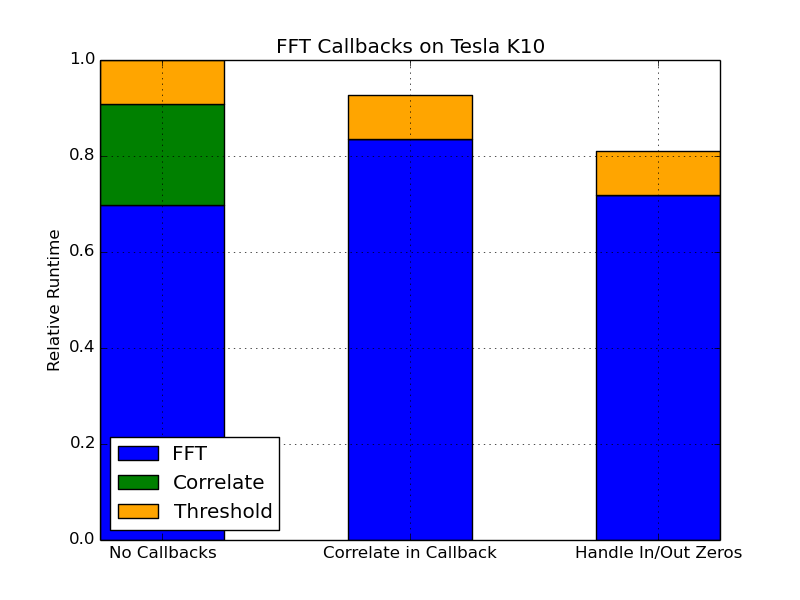
\includegraphics[width=0.6\textwidth]{callback.png}
%\caption{\label{fig:callback} 
%The relative performance of the kernels that make up the critical inner %loop of the 
%matched-filtering code. Shorter bars represent better performance. Left: The initial GPU kernel implementations without the
%use of cuFFT callbacks. Middle: Naive fusion of the correlate into a load callback.
%Right: Fusion of the correlate kernel into the load callback, where memory reads
%are avoided where the input is known to be zeros, and output writes are avoided
%where it is known to be corrupted by wrap-around effects. It is not currently
%possible to fuse the threshold kernel into the FFT, however we are working
%with NVIDIA to make the necessary changes to the cuFFT callback API to further
%optimize the code.
%}
%\end{SCfigure}

More optimal use of the available memory bandwidth can also be achieved by
reducing the amount of data sent over the memory bus. We are investigating the
possibility of storing the output SNR time and input template phase as
half-precision (FP16) numbers to reduce memory bandwidth. We have also
discussed with NVIDIA the possibility of adding callbacks to the intermediate
steps of the cuFFT implementation (since our $2^{20}$ point FFTs are
implemented by three kernel calls in cuFFT) that would allow us to use FP16
precision between each FFT radix. Performing the FFT operations
in FP32 and storing the intermediate products in FP16 may be possible. We are beginning
a study to determine if this model could meet our accuracy requirements.

Finally, we are investigating the optimal GPU/CPU ratio for systems and
parellization between the host CPU and GPU kernel execution. As GPU kernel
launches are asynchronous compared to host execution, it is possible to hide
trivial serial operations that occur within the host code. The exception is
where triggers are offloaded from the GPU onto the CPU, which is a blocking
operation. Host execution does not proceed until the GPU queue is drained.
When the data is synchronized there is a noticeable delay before new GPU
kernels are executing. This can be minimized by executing multiple host
processes that submit work to the same GPU, and by batching additional work
together to amortize the device offload latency. We have shown that two
processes running on the same CPU launching kernels to a single GPU makes more
efficient use of the GPU resources; tests to find the optimal ratio are
ongoing.

\vspace*{-10pt}
\subsection{CPU Hardware Trade Study}
\vspace*{-05pt}
\label{sec:cpu-trade}

We have benchmarked the current best implementation of the
\texttt{pycbc\_inspiral} executable several different CPU systems and studies
are ongoing to determine the most cost-effective CPU configuration for the
high-latency CBC search. Benchmarking was performed on a dedicated machine,
with all cores occupied with the CBC search code to simulate production use
(either in single-thread or multi-thread mode). For FFTW benchmarking, plans
were measured using the patient measure level for the appropriate hardware.
Table~\ref{tab:cpu-trade-study} shows the benchmarking results for the Intel
Westmere, Sandybridge, Ivybridge, and Haswell CPUs that we have tested to
date. Similar to the low-latency results, the fastest throughput is obtained
on the Intel E5-1660-v3 Haswell processor. One interesting result we note
is that the fastest throughput per \emph{active} core is obtained on a 10 core
Ivybridge E5-2670 v2 CPU when FFTW is run with two cores disabled. This also
yields a slightly faster throughput per socket, even when we account for the
fact that we are paying for two disabled cores. We attribute this to the fact
that FFTW achieves better performance with power-of-two numbers of cores, and
the E5-2670 v2 has a 25~MB level 3 cache, and so at the 4096~Hz sample rate,
almost all of the data (correlation and FFT) fits into cache. We are
continuing to explore different CPU clock speed, cache size, and cores per
socket configurations to determine the best throughput, although this also
involves writing PyCBC CPU kernels specific to e.g. AVX2 instructions to
obtain best performance. These optimization efforts are ongoing as part of our
software improvements and hardware trade study.

\begin{table}[!t]
\begin{center}
{\small
\begin{tabular}{|l|c|c|c|c|c|c|l|}
\hline
Processor   & Base clock  & cores /    & Level 3  & LIGO Data  & \multicolumn{2}{c|}{Search Throughput} & FFT Engine \\
            & speed       & socket     & Cache    & sample rate          &  \multicolumn{2}{c|}{(templates/active core)}&            \\
            & (GHz)       &            & (MB)     &  (Hz)                  &   Type A Data  & Type C Data  &            \\
\hline

E5-1660 v3  & 3.0 & 8          & 20 MB         & 4096          &  9603 &  7395 & FFTW 8 thread      \\
E5-2670 v2  & 2.5 & 10         & 25 MB         & 4096          &  8211 &  4398 & FFTW 8 thread     \\
E5-2640 v3  & 2.6 & 8          & 20 MB         & 4096          &  8131 &  6162 & FFTW 8 thread      \\
E3-1220 v3  & 3.1 & 4          & 8 MB          & 4096          &  7402 &  6579 & MKL 1 thread       \\
E3-1241 v3  & 3.5 & 4          & 8 MB          & 4096          &  7351 &  6225 & FFTW 4 thread      \\
E3-1220 v3  & 3.1 & 4          & 8 MB          & 4096          &  6842 &  5497 & FFTW 4 thread      \\
E5-2670 v2  & 2.5 & 10         & 25 MB         & 4096          &  6395 &  3523 & FFTW 10 thread     \\
E5-2670     & 2.6 & 8          & 20 MB         & 4096          &  6390 &  3673 & FFTW 8 thread      \\
E5-2670     & 2.6 & 8          & 20 MB         & 4096          &  5878 &  3606 & MKL 1 thread       \\
X5650       & 2.66 & 6         & 12 MB         & 4096          &  4320 &  3264 & MKL 1 thread       \\\hline\hline
% FIXME: check these numbers, they don't make sense

E3-1220 v3  & 3.1 & 4          & 8 MB          & 2048          & 17952 & 12394 & FFTW 4 thread      \\
E3-1220 v3  & 3.1 & 4          & 8 MB          & 2048          & 15226 & 11834 & MKL 1 thread       \\
E5-2670     & 2.6 & 8          & 20 MB         & 2048          & 15025 &  6508 & FFTW 8 thread      \\
E5-2670     & 2.6 & 8          & 20 MB         & 2048          & 10414 &  6306 & MKL 1 thread       \\
X5650       & 2.66 & 6          & 12 MB         & 2048          &  8230 &  5472 & MKL 1 thread       \\\hline
\end{tabular}  
}
\caption{%
\label{tab:cpu-trade-study}
Comparison of \texttt{pycbc\_inspiral} throughput on different Intel Westmere
(X5650), Sandybridge (E5-2670), Ivybridge (E5-2670 v2), and Haswell (E3-1220 v3,
E5-1660 v3, E5-2640 v3, and E3-1241 v3)
CPUs. Search throughput is given in templates per active socket used in the
FFT. We also show the throughput for two different input data sample rates,
4096~Hz (as used in the S6/VSR2,3 analysis) and 2048~Hz, to illustrate the
effect of Level 3 cache size on the throughput. We note that the fastest
throughput per active socket is from the 10-core Ivybridge processor with 
eight-core multi-threaded FFTW. We attribute this to the increased size of the
cache (25 MB) and the effect of non-power-of-two transforms. For a cost
metric, we should compute the throughput per socket, however even with this
metric the E5-2670 v2 CPU is faster when run in 8-core mode than in 10-core
mode (65,680 vs 63,950 E5-2670 v2 templates per socket). We also note that for
the cheaper E3-1220 v3 Haswell with an 8~MB Level 3 cache, single-threaded MKL yields the fastest throughput. 
 We also note that the code used has been optimized to the Sandybridge
architecture, and further optimization to the Haswell architecture may be
possible.
These comparisons illustrate the type of
considerations that we are exploring to determine the most cost effective
hardware.
}
\end{center}
\end{table}

\vspace*{-10pt}
\section{Comparison of LALApps and PyCBC Profiling}
\vspace*{-05pt}
\label{a:lalapps}

In this appendix we provide complete profiling for the
\texttt{lalapps\_inspiral} executable used to estimate computational cost for
May 2014 review and the new \texttt{pycbc\_inspiral} executable used in the
current estimate. The benchmarked speed for \texttt{lalapps\_inspiral} quoted
in the May 2014 review was 756 templates per E5-2670 core. We have
re-benchmarked the \texttt{lalapps\_inspiral} code to confirm these numbers
and obtain, when averaging over the three data types A, B, and C, a throughput
of 788 templates per E5-2670 core, consistent with the performance measured in
April 2014. Table~\ref{tab:lalapps-inspiral-mkl} shows the complete call graph
for one invocation of the retired LALApps executable. Using this information, we
identified the time-frequency signal-based and the FFT engine as the first
targets for optimization. We used additional profiling to identify the non-FFT
parts of the code (e.g.  \texttt{LALFindChirpClusterEvents} which performs
clustering and \texttt{LALFindChirpFilterSegment} which performs correlation
and thresholding) that were causing performance bottlenecks in the use of
parallel FFTs. For comparison, we show the current \texttt{pycbc\_inspiral}
executable run on the same data and template bank, using eight-thread FFTW.
The improvements that we have made cause the total execution time to drop so
significantly  (from 3556 seconds to 140 seconds) that the profile information
is dominated by the data reading and pre-conditioning, as shown in
Table~\ref{tab:pycbc-small-job}.  To ensure that the matched filtering
dominates the profiling and throughput measurement of
\texttt{pycbc\_inspiral},
we have run all other \texttt{pycbc\_inspiral} tests on significantly larger template banks than the
\texttt{lalapps\_inspiral} executable was able to process (57,222 templates per
bank compared to 2469  in May 2014).

\begin{table}[!b]
{\scriptsize
\begin{verbatim}
CPU: Intel Sandy Bridge microarchitecture, speed 2600.04 MHz (estimated)
Counted CPU_CLK_UNHALTED events (Clock cycles when not halted) with a unit mask of 0x00 (No unit mask) count 100000
%        total time   image name               symbol name
31.179   2084.289   liblalinspiral.so.9.0.0    Chisq_CPU
16.502   1103.165             libmkl_avx.so    mkl_dft_avx_ipps_cFft_BlkSplit_32fc
11.120    743.379             libmkl_avx.so    mkl_dft_avx_ipps_cFft_BlkMerge_32fc
5.896    394.141              libc-2.12.so    __GI_memset
5.801    387.804             libmkl_avx.so    anonymous
4.232    282.916             libmkl_avx.so    mkl_dft_avx_ipps_cFftInv_Fact4_32fc
4.139    276.692             libmkl_avx.so    anonymous
4.027    269.185             libmkl_avx.so    anonymous
3.987    266.558             libmkl_avx.so    anonymous
2.329    155.694   liblalinspiral.so.9.0.0    XLALBankVetoCCMat
1.831    122.402             libmkl_avx.so    anonymous
1.771    118.371              libm-2.12.so    __ieee754_log
1.428     95.462             libmkl_avx.so    anonymous
1.396     93.296             libmkl_avx.so    anonymous
1.268     84.799   liblalinspiral.so.9.0.0    LALFindChirpClusterEvents
0.677     45.257                no-vmlinux    /no-vmlinux
0.663     44.315   liblalinspiral.so.9.0.0    LALFindChirpFilterSegment
0.471     31.460   liblalinspiral.so.9.0.0    LALFindChirpSPTemplate
0.277     18.511              libc-2.12.so    memcpy
0.128      8.543         libFrame.so.1.4.1    Frz_inflate_fast
0.124      8.303              libm-2.12.so    log
0.121      8.102             libmkl_avx.so    mkl_dft_avx_ipps_cFftInv_Large_32fc
0.105      7.033             libmkl_avx.so    anonymous
0.081      5.395           liblal.so.9.0.0    XLALIIRFilterREAL4Vector
0.072      4.827         libFrame.so.1.4.1    FrCksumGnu
0.049      3.249           liblal.so.9.0.0    XLALREAL4ReverseFFT
0.037      2.460             libmkl_avx.so    workaround_for_DFTInv_RPack_32f
0.033      2.173              libm-2.12.so    isnan
0.026      1.718   liblalinspiral.so.9.0.0    LALFindChirpComputeChisqBins
0.021      1.417           liblal.so.9.0.0    XLALIIRFilterREAL8Vector
0.021      1.417           liblal.so.9.0.0    XLALIIRFilterReverseREAL8Vector
0.021      1.397             libmkl_avx.so    mkl_dft_avx_ipps_cCcsRecombine_32f
\end{verbatim}
}
\caption{%
\label{tab:lalapps-inspiral-mkl}
Complete profiling information for the fastest configuration of the retired
\texttt{lalapps\_inspiral} executable used for cost estimates in May 2014. The code uses the single-threaded Intel MKL FFT engine and is run on an Intel
E5-2670. The total run-time of the code is 6685 seconds, with a total of 3556
seconds spent in the MKL FFT routines. The next largest consumer of CPU time
is the \texttt{Chisq\_CPU} function that calculates the time-frequency
signal-based veto. Improvement of this algorithm, as described in
Section~\ref{sec:opt-chisq} was our first priority for optimization.
}
\end{table}


Finally, Figures~\ref{fig:clean-callgraph} and \ref{fig:grumbly-callgraph}
show the full call profile graphs for the \texttt{pycbc\_inspiral} executable
on Type A (clean) data and Type C (non-Gaussian) data respectively. These call
graphs show profiling information for the runs used to produce the template
throughput measurements on our reference CPUs given in Eqs.~(\ref{eq:c-clean})
and (\ref{eq:c-grumbly}). The code is run on a 57,222 template bank 
so that the matched filtering dominates the run-time
of the executable.
Each box in the call graph is labeled with a Python module name, line number,
and function call on the first line. The second line shows the cumulative
percentage and, in square brackets, the absolute time in seconds spent in that
function \emph{and all of its children}. The third line shows the percentage
of time actually spent in that function as a percentage and an absolute time
in seconds. The fourth line shows how many times that function was called.
Note that when reading these call graphs, the \texttt{scipy.weave} compiled
code (including the compiler intrinsics) appears in a single function called
\texttt{$\sim$:0:<apply>}, so it is necessary to look at the parent function of
this call to determine how much time is spent in a higher-level operation.
The highest-level user-code function is the third box labeled
\texttt{pycbc\_inspiral:19:<module>}.  Clearly, 100\% of the time will spent
in that function and its children, since it is the main program. However, only
1.39\% of the total execution time is spent actually in that module. In the
Type A (clean) data shown in Figure~\ref{fig:clean-callgraph} the FFT engine
dominates the computation cost, with the correlation used to compute the
integrand of the matched filter the second dominant function at 15\% of the
run-time. In the Type C data, significantly more time is spent computing the
time-frequency $\chi^2$ signal-based veto; this is our next target for 
optimization. 

\noindent\makebox[\linewidth]{\rule{\textwidth}{1pt}} 

%One addition result that can be seen from these call graphs is
%that the overhead of using Python is not a significant bottleneck inside the
%\textsc{findchirp} loop. For example, in the matched filter correlate
%function in Figure~\ref{fig:clean-callgraph}, computing the total ratio of the time
%spent in \texttt{matchedfilter\_cpu:93:correlate} to its children shows that
%only 1.5\% of the total time in this function is Python overhead.


\begin{table}[!b]
{\scriptsize
\begin{verbatim}
ncalls  total time  filename:lineno(function)
37035   55.188      fftw.py:451(execute)
92301   32.677      {apply}
1       22.851      {scipy.signal.sigtools._linear_filter}
1        8.896      {_lalframe.FrStreamReadREAL8TimeSeries}
1        2.506      {_lal.HighPassREAL8TimeSeries}
\end{verbatim}
}
\caption{%
\label{tab:pycbc-small-job}
The \texttt{pycbc\_inspiral} executable run on the same input data and
template bank as shown for \texttt{lalapps\_inspiral}  in
Table~\ref{tab:lalapps-inspiral-mkl}. The PyCBC code is so much faster that
the data reading and conditioning are a significant fraction of the run-time.
To ensure that the matched filtering dominates the profiling of
\texttt{pycbc\_inspiral} we run on significantly larger template banks than
the \texttt{lalapps\_inspiral} executable was able to process, as shown in
Figures~\ref{fig:clean-callgraph} and \ref{fig:grumbly-callgraph}.
}
\end{table}

%\begin{figure}[!p]
%\centering
%\includegraphics[height=0.9\textheight]{fc3c08a_cpu_4096_one_per_socket_clean.png}
%\caption{\label{fig:clean-callgraph}
%Call graph generated for the \texttt{pycbc\_inspiral} profiling run on Type A
%(clean) data. The total run time to process the data through the template bank
%is 2158 seconds. 60\% of the total run-time is spent in the FFT engine (1304
%seconds) and 25\% of the run time is spent in the \texttt{scipy.weave.apply}
%function that calls the low-level kernels for template generation,
%correlation, the time-frequency signal-based vetoes, and thresholding and
%clustering.
%}
%\end{figure}

%\begin{figure}[!p]
%\centering
%\includegraphics[height=0.9\textheight]{fc3c08a_cpu_4096_one_per_socket_grumbly.png}
%\caption{\label{fig:grumbly-callgraph}
%Call graph generated for the \texttt{pycbc\_inspiral} profiling run on Type C
%(very non-Gaussian) data. The total run time to process the data through the template bank
%is 3583 seconds. Now 32\% of the total run-time is spent in the FFT engine (1158
%seconds) vs 55\% of the run time (1965 seconds)  in the
%\texttt{scipy.weave.apply} function. The change in ratio and increase in run-time
%is due to the larger number of signal-based veto calculations
%that need to be performed; Notice that 43\% of the runtime (1541 seconds) is
%spent in the \texttt{chisq\_cpu} function and its children.
%}
%\end{figure}

\section{Development and Simulation Costs}
\vspace*{-5pt}

The May 2014 request for computational resources presented in LIGO-T1400269
presented the total production computing request, but it did not include an
estimate of the computational resources needed to develop, test, and tune the
searches prior to the observing runs. For completeness in this appendix, we
present our best estimate of the resources needed to develop and test the
high-latency CBC search before the observing runs, using the measured
throughput for the best optimized \texttt{pycbc\_inspiral}. The request in MSU
is for all high-latency CBC computing summarized in
Table~\ref{t:offline-xsede-all}. Resources needed for development are larger
relative to production in the earlier epochs. This is due to the fact that
more time is spent in engineering runs, mock data challenges, and development
and reduce in later years as more time is spent in observing runs. The
requested time for simulations includes the computational resources necessary
to review the analyses prior to observing runs. 

To obtain development costs, we assume that the detectors will be operating
with a 20\% duty cycle between observing runs. This time will comprise
engineering runs as well as night and weekend running when the detector is in
a sufficiently stable state during commissioning to record data. We assume
that only three sets of tuning injections are performed. The simulation
request is based on experience with the number of mock data challenges needed
to prepare for O1: we expect to analyze approximately 3 months of data between
O1 and O2, and 1.5 months of data between O2 and O3 in mock data challenges.
However, the actual costs will be updated based on experience.

\begin{table}[!h]
\centering
{\small
\begin{tabular}{|l|l|l|l|}
\hline 
{\bf Astrophysical search target}  & \multicolumn{3}{l|}{\bf E5-2670 MSU per year}\\

{ } &  {\bf 2015--16} & {\bf 2016--17} & {\bf 2017--18}  \\\hline\hline
{ Production:\, Binary neutron stars (non-spinning)} & 0.084 & 0.514 & 1.48 \\\hline
{ Production: Binary neutron stars (aligned-spin)} & 1.25 & 8.82 & 30.2 \\\hline
{ Development and Simulation: Binary neutron stars (non-spinning) } &  0.169 &  0.218 &  0.110 \\\hline
{ Development and Simulation: Binary neutron stars (aligned-spin) } &  2.49 &  3.70 &  2.21 \\\hline\hline
{ Production: Neutron star--black hole (aligned spin) } & 2.26 & 17.5 & 65.7 \\\hline
{ Development and Simulation: Neutron star--black hole (aligned spin) } &  4.52 & 7.32 & 4.76 \\\hline\hline
{ Production: Binary black hole search  (aligned spin) } &1.45 & 11.9 & 36.1 \\\hline
{ Development and Simulation: Binary black hole search  (aligned spin) } & 1.54 & 3.28 & 1.93 \\\hline\hline
{ \bf Total for high-latency CBC development, simulation, and production } & \bf 13.8 & \bf 53.3 & \bf 143 \\\hline
\end{tabular}
}
\caption{\label{t:offline-xsede-all}
The total computational resources needed for production, simulations, and
development for the high-latency CBC search in millions of service units (MSU) per
year. One service unit is defined as one core hour on an Intel\textsuperscript{\textregistered} 
E5-2670.  The production request is identical to the request in Table~\ref{t:offline-xsede-request} in this document. The development and simulation request are our best estimates of the computational resources required to develop and tune the searches prior to the observing runs in each epoch. The total for production, simulations, and
development is reflected in the total CBC request in the LSC Computing Plan
LIGO-T1500118 (see e.g. Table 3, page 13 of LIGO-T1500118 for comparison with
the total O3 request).
%Note the non-spinning binary neutron star search is a sub-set of the
%aligned spin binary neutron star search, so only one of these searches will be
%performed. 
%Shown below each science goal (in italics) is the size of the
%corresponding May 2014 request from Table 3 of LIGO-T1400269; the difference from May 2014 to April 2015 reflect optimization of code and the flow down of science priorities. Since no search
%pipeline for precessing searches exists, this search is currently not listed
%in the LSC's prioritized science goals.  Large-scale simulations included in
%the above cost will allow us to measure the sensitivity of aligned-spin
%searches to precessing systems.
}
\end{table}
